\documentclass[a5paper]{article}
\usepackage[a5paper, top=8mm, bottom=8mm, left=8mm, right=8mm]{geometry}

\usepackage{polyglossia}
\setdefaultlanguage[babelshorthands=true]{russian}

\usepackage{fontspec}
\setmainfont{FreeSerif}
\newfontfamily{\russianfonttt}[Scale=0.7]{DejaVuSansMono}

\usepackage[font=scriptsize]{caption}

\usepackage{amsmath}
\usepackage{amssymb,amsfonts,textcomp}
\usepackage{color}
\usepackage{array}
\usepackage{hhline}
\usepackage{cite}
\usepackage{textcomp}

\usepackage[hang,multiple]{footmisc}
\renewcommand{\footnotelayout}{\raggedright}

\PassOptionsToPackage{hyphens}{url}\usepackage[xetex,linktocpage=true,plainpages=false,pdfpagelabels=false]{hyperref}
\hypersetup{colorlinks=true, linkcolor=blue, citecolor=blue, filecolor=blue, urlcolor=blue, pdftitle=1, pdfauthor=, pdfsubject=, pdfkeywords=}

\newlength\Colsep
\setlength\Colsep{10pt}

\usepackage{tabu}

\usepackage{graphicx}
\usepackage{indentfirst}
\usepackage{multirow}
\usepackage{subfig}
\usepackage{footnote}
\usepackage{minted}

\newcommand{\attribution}[1] {
    \vspace{-5mm}\begin{flushright}\begin{scriptsize}%\textcolor{gray}
    {\textcopyright\, #1}\end{scriptsize}\end{flushright}
}

\sloppy
\pagestyle{plain}

\title{Лекция 5:  Моделирование поведения}
\author{Юрий Литвинов\\\small{yurii.litvinov@gmail.com}}
\date{07.03.2022}

\begin{document}

\maketitle
\thispagestyle{empty}

\section{Введение}

В этой лекции мы закончим обсуждение UML, рассмотрев диаграммы, которые используются на этапе разработки, или более конкретно, для моделирования поведения. Речь пойдёт не только про UML, но и некоторые другие формализмы, используемые для этой цели.

\section{Диаграммы конечных автоматов}

Диаграммы конечных автоматов (также известные как диаграммы состояний) --- это на самом деле несколько упрощённые диаграммы Харела, предложенные им ещё в 1987 году, которые попали в UML с минимальными изменениями. Это второй вид диаграмм UML, имеющий исполнимую семантику (первый --- диаграммы активностей, которые были рассмотрены в предыдущей лекции). Предназначены эти диаграммы для моделирования поведения <<реактивных>> систем (или частей системы), то есть систем, которые находятся в некоторых чётко определённых состояниях, от которых зависит их поведение, и могут реагировать на события, переходя из состояния в состояние и, возможно, делая при переходах полезную работу. Примеры реактивных систем --- это сетевое соединение (которое может быть открыто, закрыто, открываемо в данный момент, закрываемо, и в зависимости от этого передаёт или не передаёт пакеты), либо классический пример с торговым автоматом, с которого начинался рассказ про моделирование вообще.

Выглядят диаграммы конечных автоматов так:

\begin{center}
    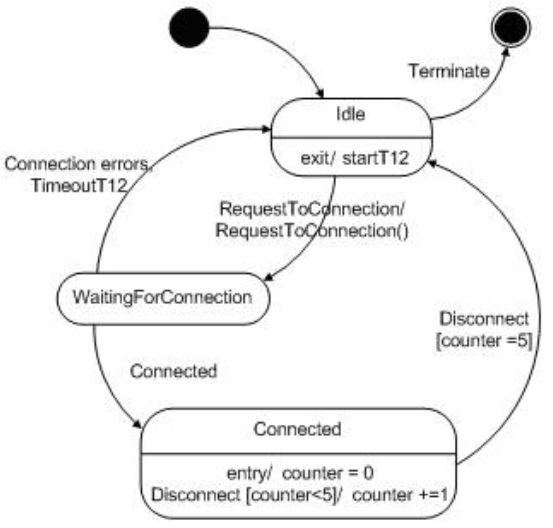
\includegraphics[width=0.4\textwidth]{stateTransitionExample.png}
\end{center}

Прямоугольниками со скруглёнными углами рисуются состояния, у состояния есть имя и (опционально) действия, выполняемые в состоянии (например, действие по выходу или внутренний переход по событию, как у Connected --- получив событие Disconnect, оно проверяет счётчик, и если счётчик меньше 5, он увеличивается на 1 и мы остаёмся в том же состоянии). Состояния связаны переходами, над переходом пишется событие, которое инициирует переход и, опционально, стражник (guard) (логическое условие, которое должно быть истинно, чтобы переход состоялся) и действие, выполняемое при переходе. События со стражниками должны быть взаимно исключающими, недетерминированные автоматы считаются некорректными. Есть псевдосостояния начала и конца, переход из псевдосостояния начала происходит мгновенно, переход в состояние конца заканчивает исполнение.

Внешне диаграммы конечных автоматов похожи на диаграммы активностей, но есть важные семантические различия:

\begin{itemize}
    \item на диаграмме активностей рисуются активности, система в них не задерживается, а сразу переходит дальше; на диаграмме конечных автоматов рисуются состояния --- стабильные отрезки жизненного цикла объекта, в которых он находится большую часть времени и может из них выйти только если что-то произойдёт;
    \item полезная работа на диаграммах активностей производится в активностях, на диаграммах автоматов --- как правило, при переходе;
    \item диаграммы активностей моделируют один метод объекта (или какую-то функцию или что-то такое), диаграммы конечных автоматов --- целый объект (состояния моделируются полями объекта).
\end{itemize}

Более подробно про синтаксис:

\begin{center}
    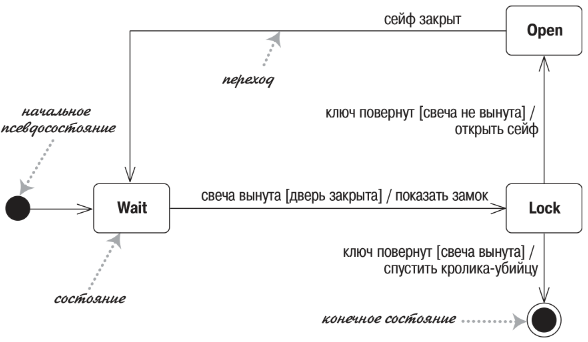
\includegraphics[width=0.7\textwidth]{stateTransitionSyntax.png}
    \attribution{М. Фаулер, UML. Основы}
\end{center}

Внутри состояния могут быть:

\begin{itemize}
    \item entry activity --- то, что делается при входе в состояние по любому из переходов;
    \item exit activity --- то, что делается при выходе из состояния по любому исходящему переходу (и входная, и выходная деятельность --- это, как правило, вызовы метода);
    \item do activity --- деятельность, выполняющаяся всегда, когда система находится в таком-то состоянии (например, попытки подключения к сети для мобильного телефона);
    \item внутренний переход --- переход по событию, который ведёт в то же состояние и не приводит к срабатыванию entry и exit activity. Переход вполне может быть полноценным переходом в то же состояние (рисуется как петля в графе), тогда entry и exit activity работают как обычно, хоть состояние и не меняется.
\end{itemize}

Событие, кстати, это нечто внешнее по отношению к системе, на что система может реагировать. Примеры событий --- действие пользователя, сетевой пакет, считывание символа (если речь идёт об автоматном лексическом анализаторе, который, кстати, хоть и несколько необычный, но тоже пример реактивной системы, которая прекрасно моделируется конечными автоматами).

Надпись на переходе имеет следующий синтаксис: \verb|[<trigger> [‘,’ <trigger>]* [‘[‘ <guard>’]’] [‘/’ <behavior-expression>]]| --- один переход может реагировать на несколько событий сразу, иметь опционального стражника (в квадратных скобках) и через слеш действие (вызов метода или отсылку к диаграмме активностей, которая поясняет, что нужно делать при переходе).

Вот более содержательный пример автомата из работ Д.В. Кознова. Пример демонстрирует порядок работы мобильного телефона, начиная с включения и ввода PIN-кода и заканчивая подключением к сети:

\begin{center}
    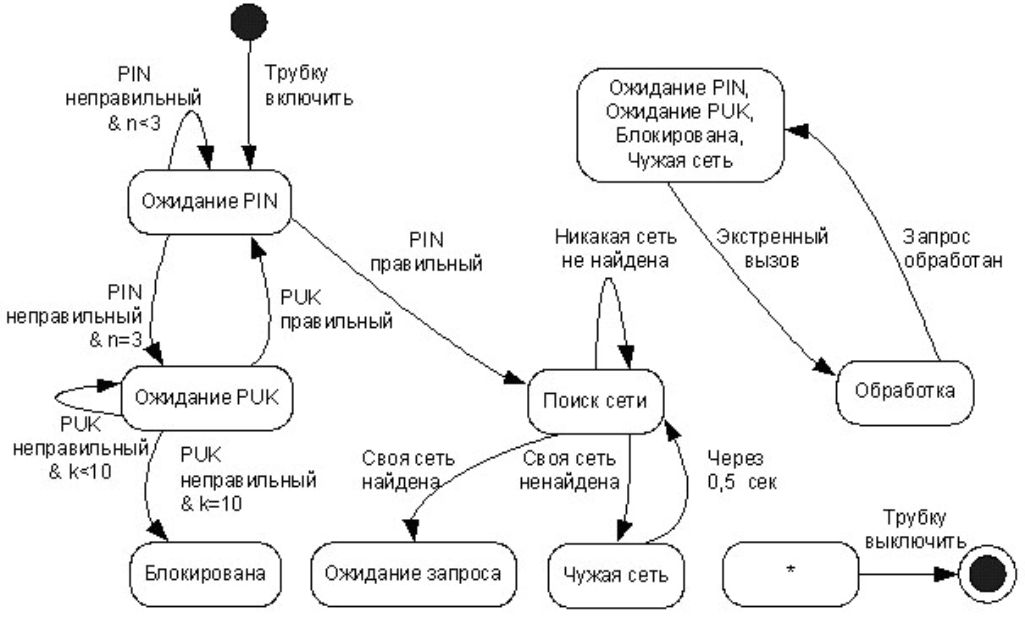
\includegraphics[width=0.7\textwidth]{stateTransitionExample2.png}
\end{center}

Тут используется неканоничный синтаксис с псевдосостоянием ``все состояния'', из которого ведёт переход в конечное псевдосостояние (чтобы не рисовать переход из каждого состояния в конечное) и используются не совсем каноничные надписи над переходами. Связано это с тем, что в те времена, когда на матмехе делались работы по диаграммам конечных автоматов, UML 2 ещё не было, а в UML первых версий синтаксис диаграмм конечных автоматов был менее проработан.

Более продвинутый синтаксис современных диаграмм конечных автоматов позволяет нарисовать пример выше более канонично. Есть вложенные состояния с переходами сразу из всех внутренних состояний:

\begin{center}
    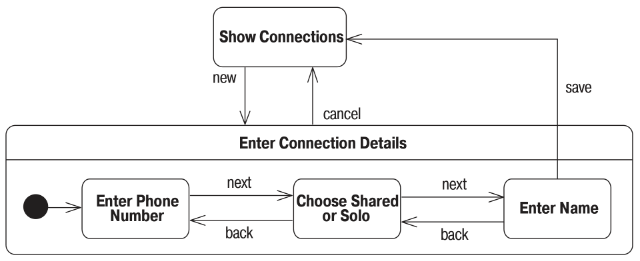
\includegraphics[width=0.7\textwidth]{stateTransitionNestedStates.png}
    \attribution{М. Фаулер, UML. Основы}
\end{center}

Тут состояние <<Enter connection details>> содержит внутри свой конечный автомат, который начинает работать со стартового псевдосостояния когда выполняется переход <<new>>. При этом переход <<save>> возможен только из состояния <<Enter Name>>, а вот переход <<cancel>> возможен из любого вложенного состояния (это замена нестандартному псевдосостоянию со звёздочкой из диаграммы выше).

Ещё бывают параллельные состояния и псевдосостояние истории:

\begin{center}
    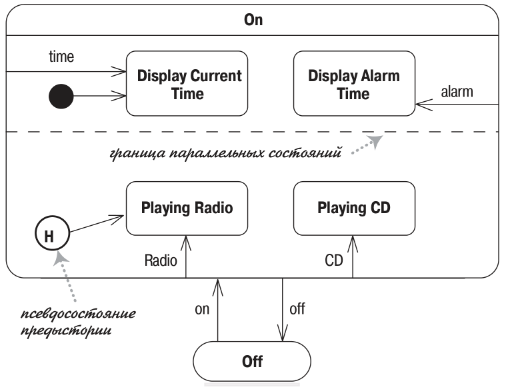
\includegraphics[width=0.6\textwidth]{stateTransitionParallelStates.png}
    \attribution{М. Фаулер, UML. Основы}
\end{center}

Это часы с радио и будильником. Проигрывание звука и время работают независимо, поэтому по сути это два автомата, работающих параллельно (что и показывает горизонтальная прерывистая линия, разделяющая параллельные подавтоматы). Стрелки от объемлющего состояния к вложенным означают, что система, находясь в объемлющем состоянии, реагирует на такие-то события и изменяет внутреннее состояние (например, часы по умолчанию показывают текущее время, но если пользователь нажал на кнопку <<будильник>>, начинает показывать время, на которое будильник установлен). Псевдосостояние истории запоминает последнее вложенное состояние, в котором находился автомат, и возвращает автомат в него. Например, часы по умолчанию включают радио, но если пользователь включил воспроизведение компакт-дисков (если кто помнит, что это такое) и выключил часы, то при следующем включении они снова будут проигрывать компакт-диски.

А вот так рисуются активности внутри состояния:

\begin{center}
    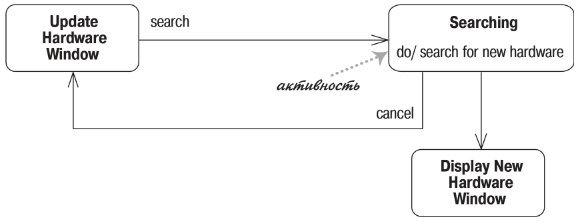
\includegraphics[width=0.6\textwidth]{stateTransitionInternalEventExample.png}
    \attribution{М. Фаулер, UML. Основы}
\end{center}

А вот так --- внутренние переходы и entry/exit-события, о которых шла речь выше:

\begin{center}
    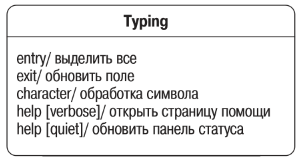
\includegraphics[width=0.35\textwidth]{stateTransitionInternalEvents.png}
    \attribution{М. Фаулер, UML. Основы}
\end{center}

Как видим, синтаксис очень похож на то, что пишется при переходе.

\subsection{Генерация кода}

Конечные автоматы хороши тем, что по ним можно легко и приятно генерировать код, в силу их стандартизованной семантики. Рассмотрим наш пример с кроликом-убийцей:

\begin{center}
    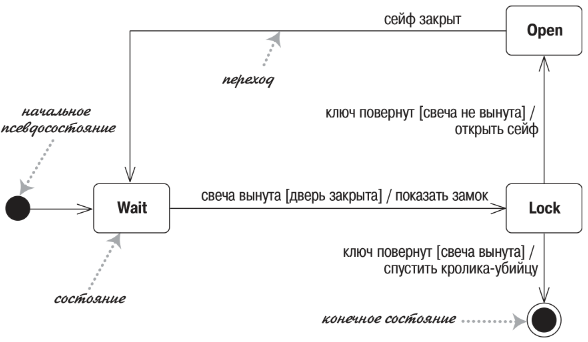
\includegraphics[width=0.8\textwidth]{stateTransitionSyntax.png}
    \attribution{М. Фаулер, UML. Основы}
\end{center}

Первый, самый простой способ сгенерировать код --- это сгенерировать гигантский switch, внутри которого чуть менее гигантские switch-и. Внешний switch --- по текущему состоянию автомата, внутренние --- по событиям, на которые находясь в данном состоянии автомат может реагировать. Внутри --- проверка условий стражников, выполнение действия по переходу и переход в следующее состояние. Состояние моделируется enum-ом, хранящимся как поле объекта. Для нашего примера получится что-то такое:

\begin{minted}{java}
public void handleEvent(PanelEvent anEvent) {
    switch (currentState) {
        case PanelState.Open:
            switch (anEvent) {
                case PanelEvent.SafeClosed:
                    currentState = PanelState.Wait;
            }
            break;
        case PanelState.Wait:
            switch (anEvent) {
                case PanelEvent.CandleRemoved:
                    if (isDoorOpen) {
                        revealLock();
                        currentState = PanelState.Lock;
                    }
            }
            break;
        case PanelState.Lock:
            switch (anEvent) {
                case PanelEvent.KeyTurned:
                    if (isCandleIn) {
                        openSafe();
                        currentState = PanelState.Open;
                    } else {
                        releaseKillerRabbit();
                        currentState = PanelState.Final;
                    }
            }
            break;
    }
}
\end{minted}

Это работает, но если этот код надо сопровождать, никто от него не будет в восторге. Для сколько-нибудь содержательных автоматов получается один метод на тысячи строк. Поэтому можно использовать таблицу состояний и универсальный интерпретатор, который просто ищет в таблице текущее состояние и событие, и выполняет то, что там написано. Вариантов таблиц состояний может быть много, но вот пример из книжки Фаулера:

\begin{center}
    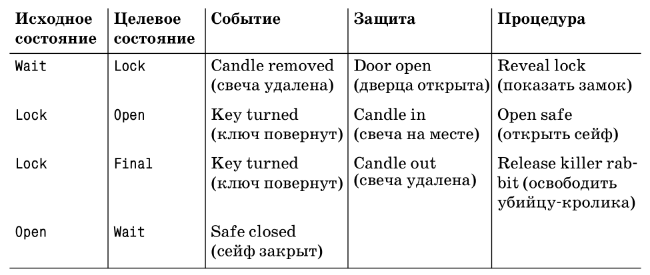
\includegraphics[width=0.6\textwidth]{stateTransitionStateTable.png}
    \attribution{М. Фаулер, UML. Основы}
\end{center}

Таблица состояний обычно либо хранится как файл данных рядом с программой, либо вкомпилируется в исходный код. 

Такой подход очень популярен в лексическом и синтаксическом анализе, но отлаживать или просто понимать такие программы очень тяжело. Поэтому есть ещё один, более объектно-ориентированный способ симулировать автомат: паттерн проектирования <<Состояние>>:

\begin{center}
    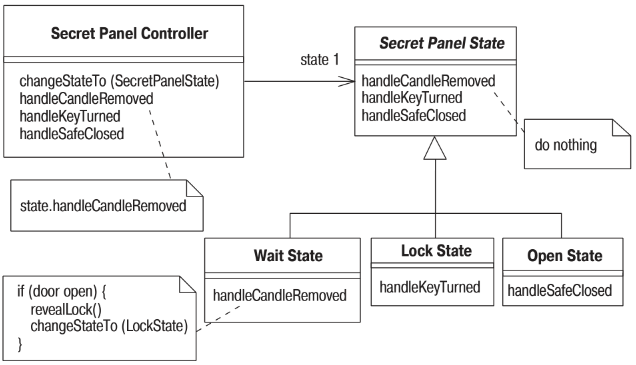
\includegraphics[width=0.6\textwidth]{stateTransitionStatePattern.png}
    \attribution{М. Фаулер, UML. Основы}
\end{center}

Автомат представляется в виде класса, который имеет в качестве поля ссылку на интерфейс <<текущее состояние>>. Этот интерфейс имеет столько методов, сколько всего разных событий может обрабатывать автомат. Интерфейс реализуют конкретные классы, отвечающие за конкретные состояния, они определяют те методы интерфейса, на которые могут реагировать, там уже проверяют условия стражников и выполняют действие при переходе. Каждый такой метод возвращает объект-состояние, в которое должен перейти автомат дальше. То есть, по сути, это тот же switch, где самый большой switch (по состояниям) спрятан в таблицу виртуальных методов. Такой подход делает реализацию автомата более-менее читаемой, ограничивает ответственность каждого класса только одним состоянием и позволяет очень легко добавить новые состояния, поэтому очень популярен при <<ручной>> реализации автоматов.

\section{Диаграммы последовательностей}

Следующий тип диаграмм UML, использующийся при моделировании поведения --- это диаграммы последовательностей (sequence diagrams). Они применяются для визуализации взаимодействия между объектами --- передачи сообщений, возврата значений, времени жизни объекта. Выглядят диаграммы следующим образом:

\begin{center}
    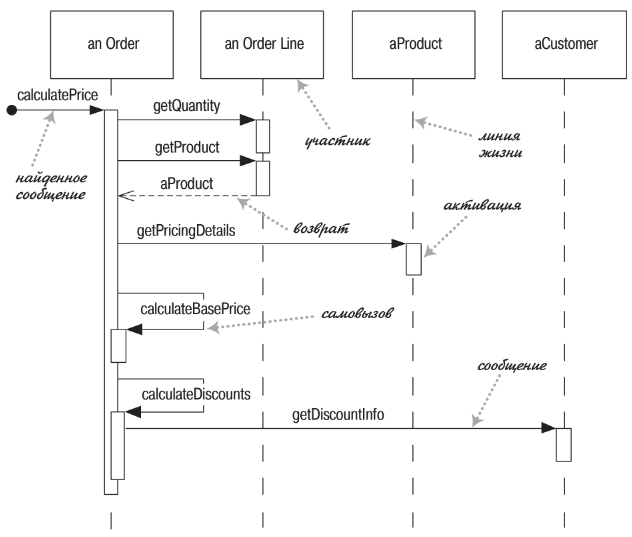
\includegraphics[width=0.8\textwidth]{sequenceDiagramSyntax.png}
    \attribution{М. Фаулер, UML. Основы}
\end{center}

На диаграмме рисуются объекты (обратите внимание, не классы), из каждого объекта выходит \textit{линия жизни} (пунктирная линия), на которой расположены \textit{линии активации} (длинный белый прямоугольник). Линия жизни показывает, когда объект вообще существует в памяти, линия активации --- когда объект занят какой-то работой (то есть работает либо его метод, либо метод, вызванный из его метода, или, более формально, какой-либо из методов объекта находится на стеке вызовов). Линий активации одновременно может быть несколько --- рекурсивные вызовы. Стрелки между линиями активации обозначают сообщения --- как правило, это вызовы методов, и поэтому они ведут в начало соответствующих вызванному методу линий активации. Обратите внимание, что стрелка не может выходить из неактивного объекта и не может входить <<в никуда>>.

Такая диаграмма позволяет разобраться в даже довольно сложных протоколах взаимодействия, поэтому применяется при многопоточном и асинхронном программировании, чтобы визуализировать общение между потоками/асинхронные вызовы. Также такие диаграммы очень популярны при описании телекоммуникационных протоколов (на самом деле, есть отдельный язык MSC (Message Sequence Charts), который применяется независимо от UML, но диаграммы последовательностей являются его почти копией).

Имеется и ряд менее очевидных применений: 

\begin{itemize}
    \item на этапе анализа предметной области для визуализации последовательности коммуникаций между участниками взаимодействия;
    \item на этапе проектирования для составления плана тестирования --- кто в каком порядке кого должен дёргать и кто когда чем должен отвечать;
    \item на этапе отладки, для визуализации логов работающей системы.
\end{itemize}

Ещё немного синтаксических подробностей:

\begin{center}
    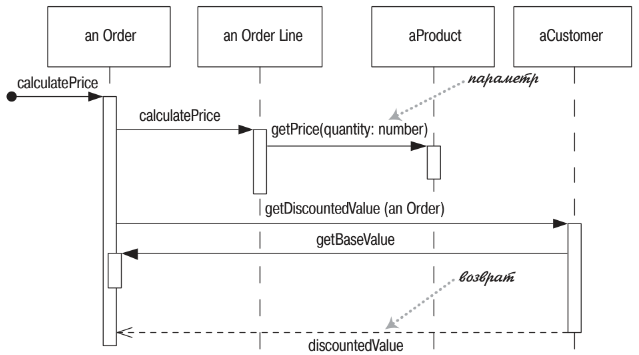
\includegraphics[width=0.7\textwidth]{sequenceDiagramSyntax2.png}
    \attribution{М. Фаулер, UML. Основы}
\end{center}

На этом примере видна передача параметров в сообщении (обратите внимание, что параметрами могут быть сами участники взаимодействия, например, <<an Order>> передаётся в <<aCustomer>>, тот самый <<an Order>>, из линии активации которого выходит сообщение). Здесь же показан возврат значения из вызова, <<discountedValue>>.

\subsection{Примеры}

Пример диаграммы последовательностей из реального проекта:

\begin{center}
    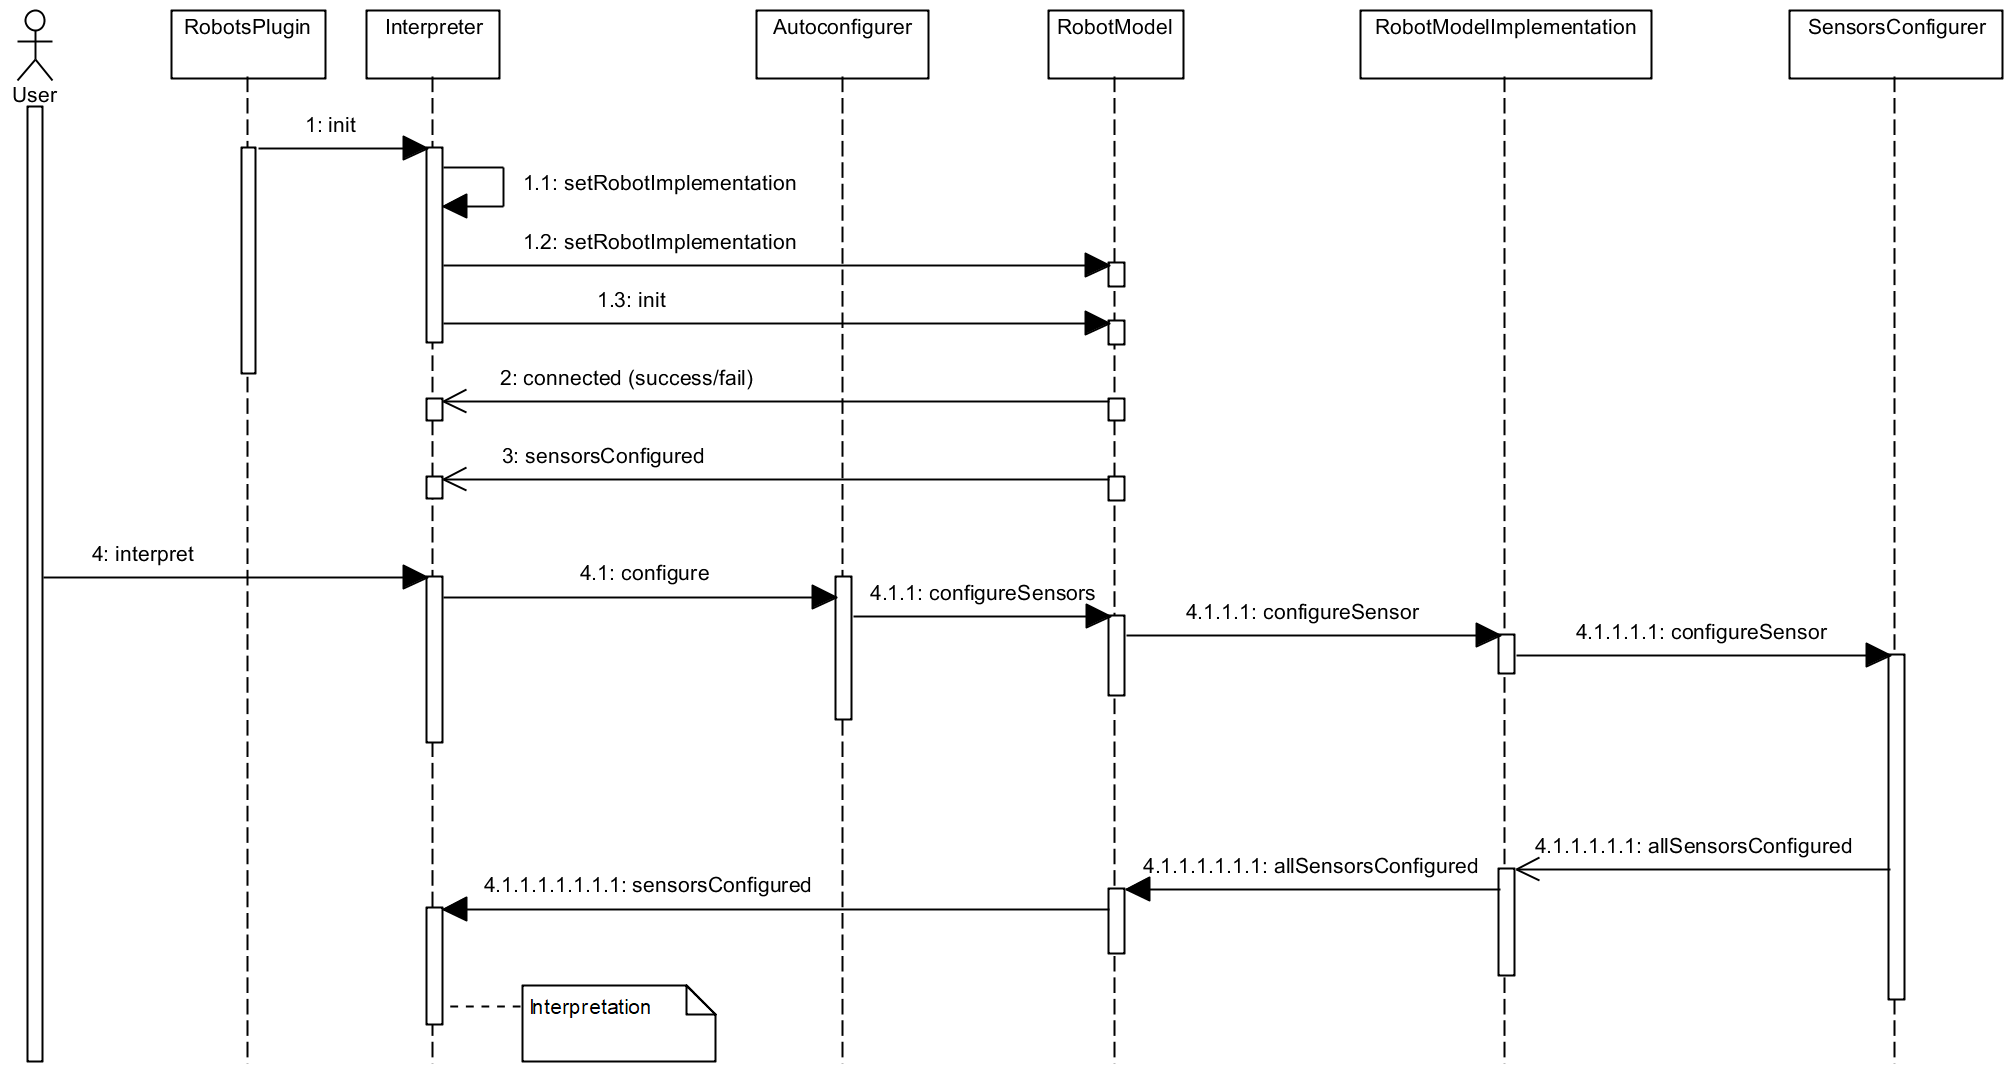
\includegraphics[width=\textwidth]{sequenceDiagramExample.png}
\end{center}

Показывается сценарий конфигурирования робота при запуске интерпретации программы в среде программирования роботов. Сначала система инициализируется, выбирает реализацию подсистемы связи с роботом (исходя из того, с каким роботом сейчас работает пользователь), посылает ему команду инициализации, после чего асинхронно получает два сигнала --- подключение удалось/не удалось (<<connected>>) и сенсоры сконфигурированы на роботе в конфигурации по умолчанию (<<sensorsConfigured>>). Далее становится доступна кнопка <<Interpret>>, пользователь нажимает её и запускает процесс конфигурации сенсоров --- среда программирования смотрит на программу, понимает, какие сенсоры и как там используются, смотрит на настройки и рассчитывает итоговую конфигурацию сенсоров, которые и шлёт на робот. Дальше она дожидается асинхронного ответа о том, что все сенсоры готовы к работе, и начинает собственно интерпретацию программы. Как видим, протокол инициализации довольно сложен, но на диаграмме он вполне обозрим, и это очень помогает при отладке.

Ещё один пример:

\begin{center}
    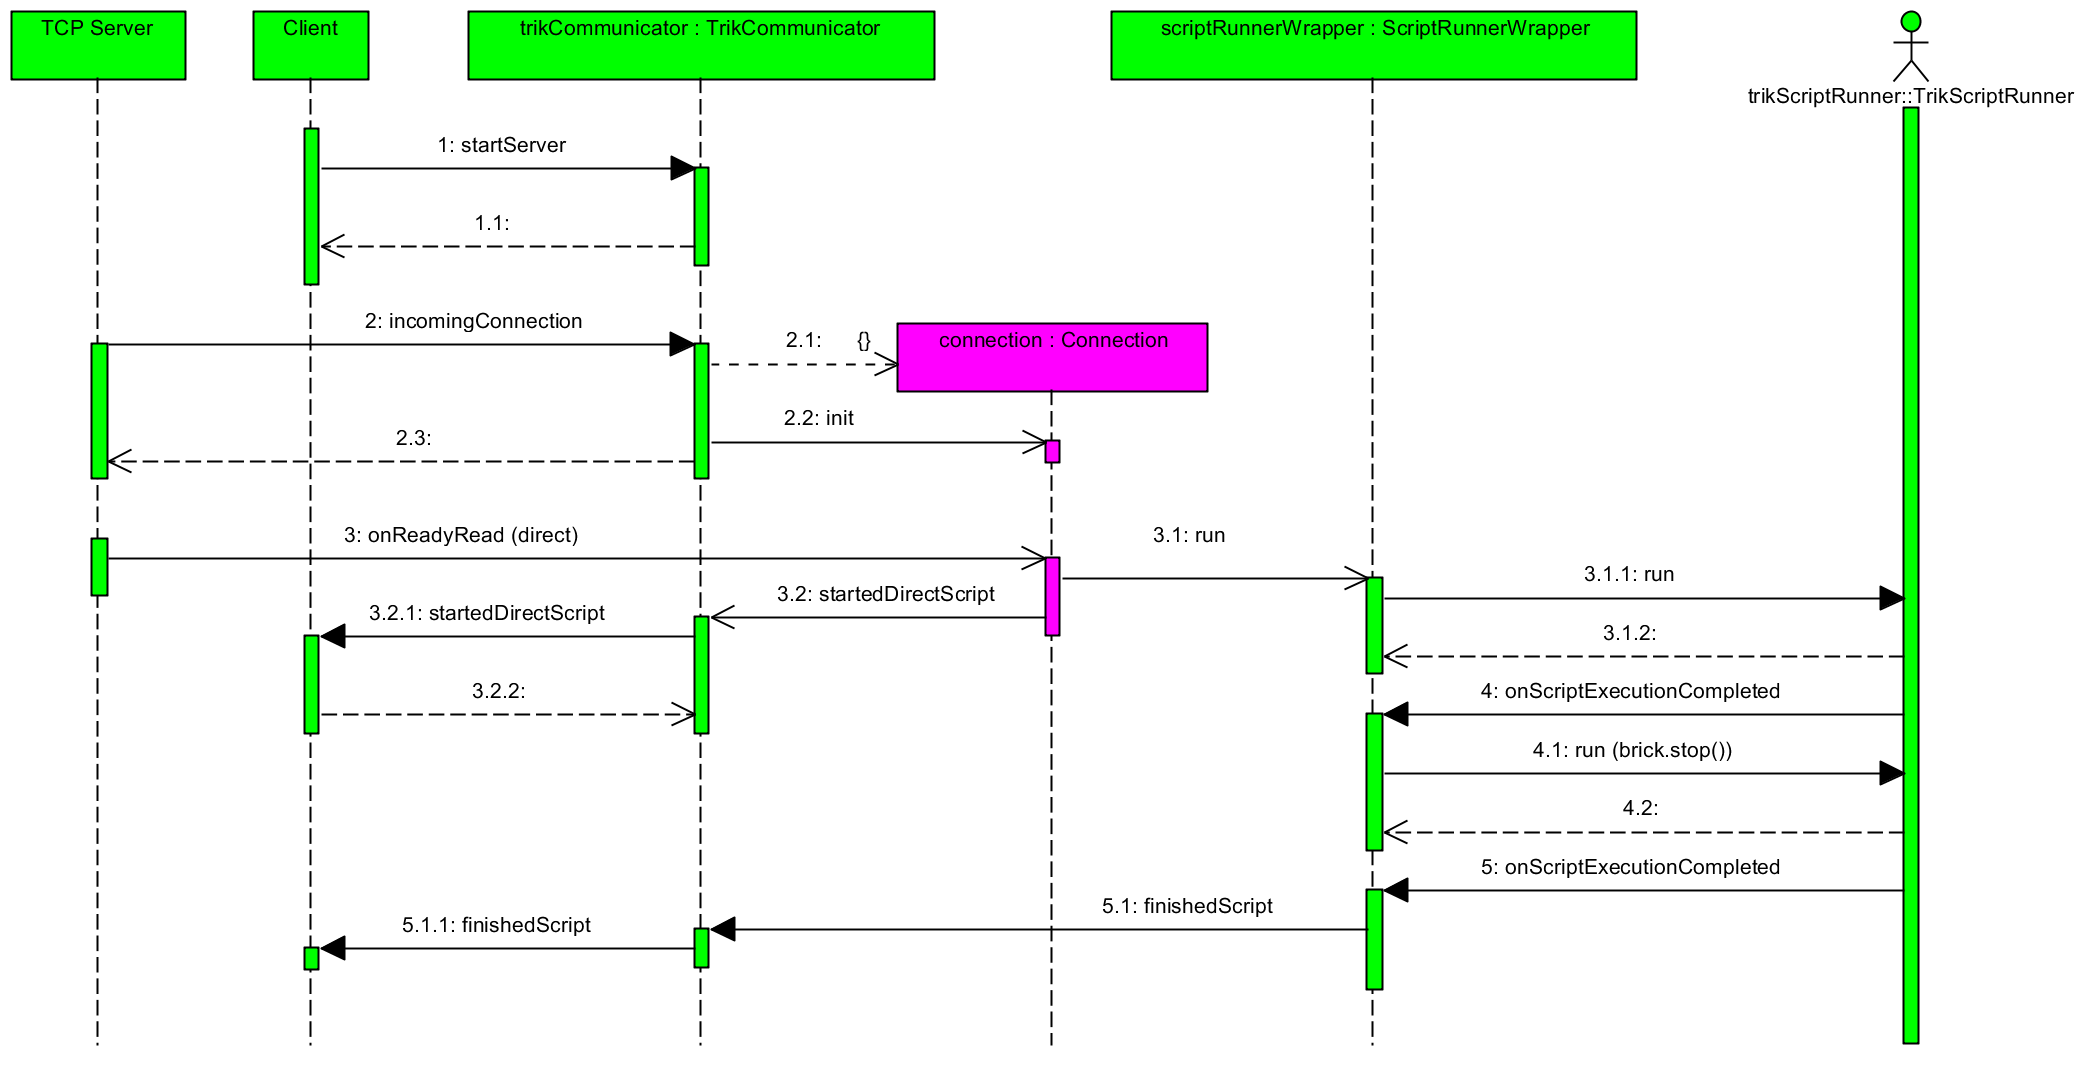
\includegraphics[width=\textwidth]{sequenceDiagramExample2.png}
\end{center}

На сей раз это сценарий выполнения скрипта на роботе. Скрипт получается по сети, для чего сначала запускают сервер, ждут входящего соединения, создают в отдельном потоке объект для его обработки, и, как только скрипт полностью загружен, запускают его на исполнение. Когда скрипт заканчивает работу, мы получаем сигнал <<onScriptExecutionCompleted>>, после чего запускаем специальный скрипт остановки робота, который должен остановить все моторы и выключить все датчики. Уже после окончания этого скрипта мы посылаем клиенту сигнал о том, что всё закончилось.

В этом примере цветом выделен объект, живущий в отдельном потоке, стандарт UML этого не предписывает (но и не запрещает), на практике очень удобно.

И ещё один пример:

\begin{center}
    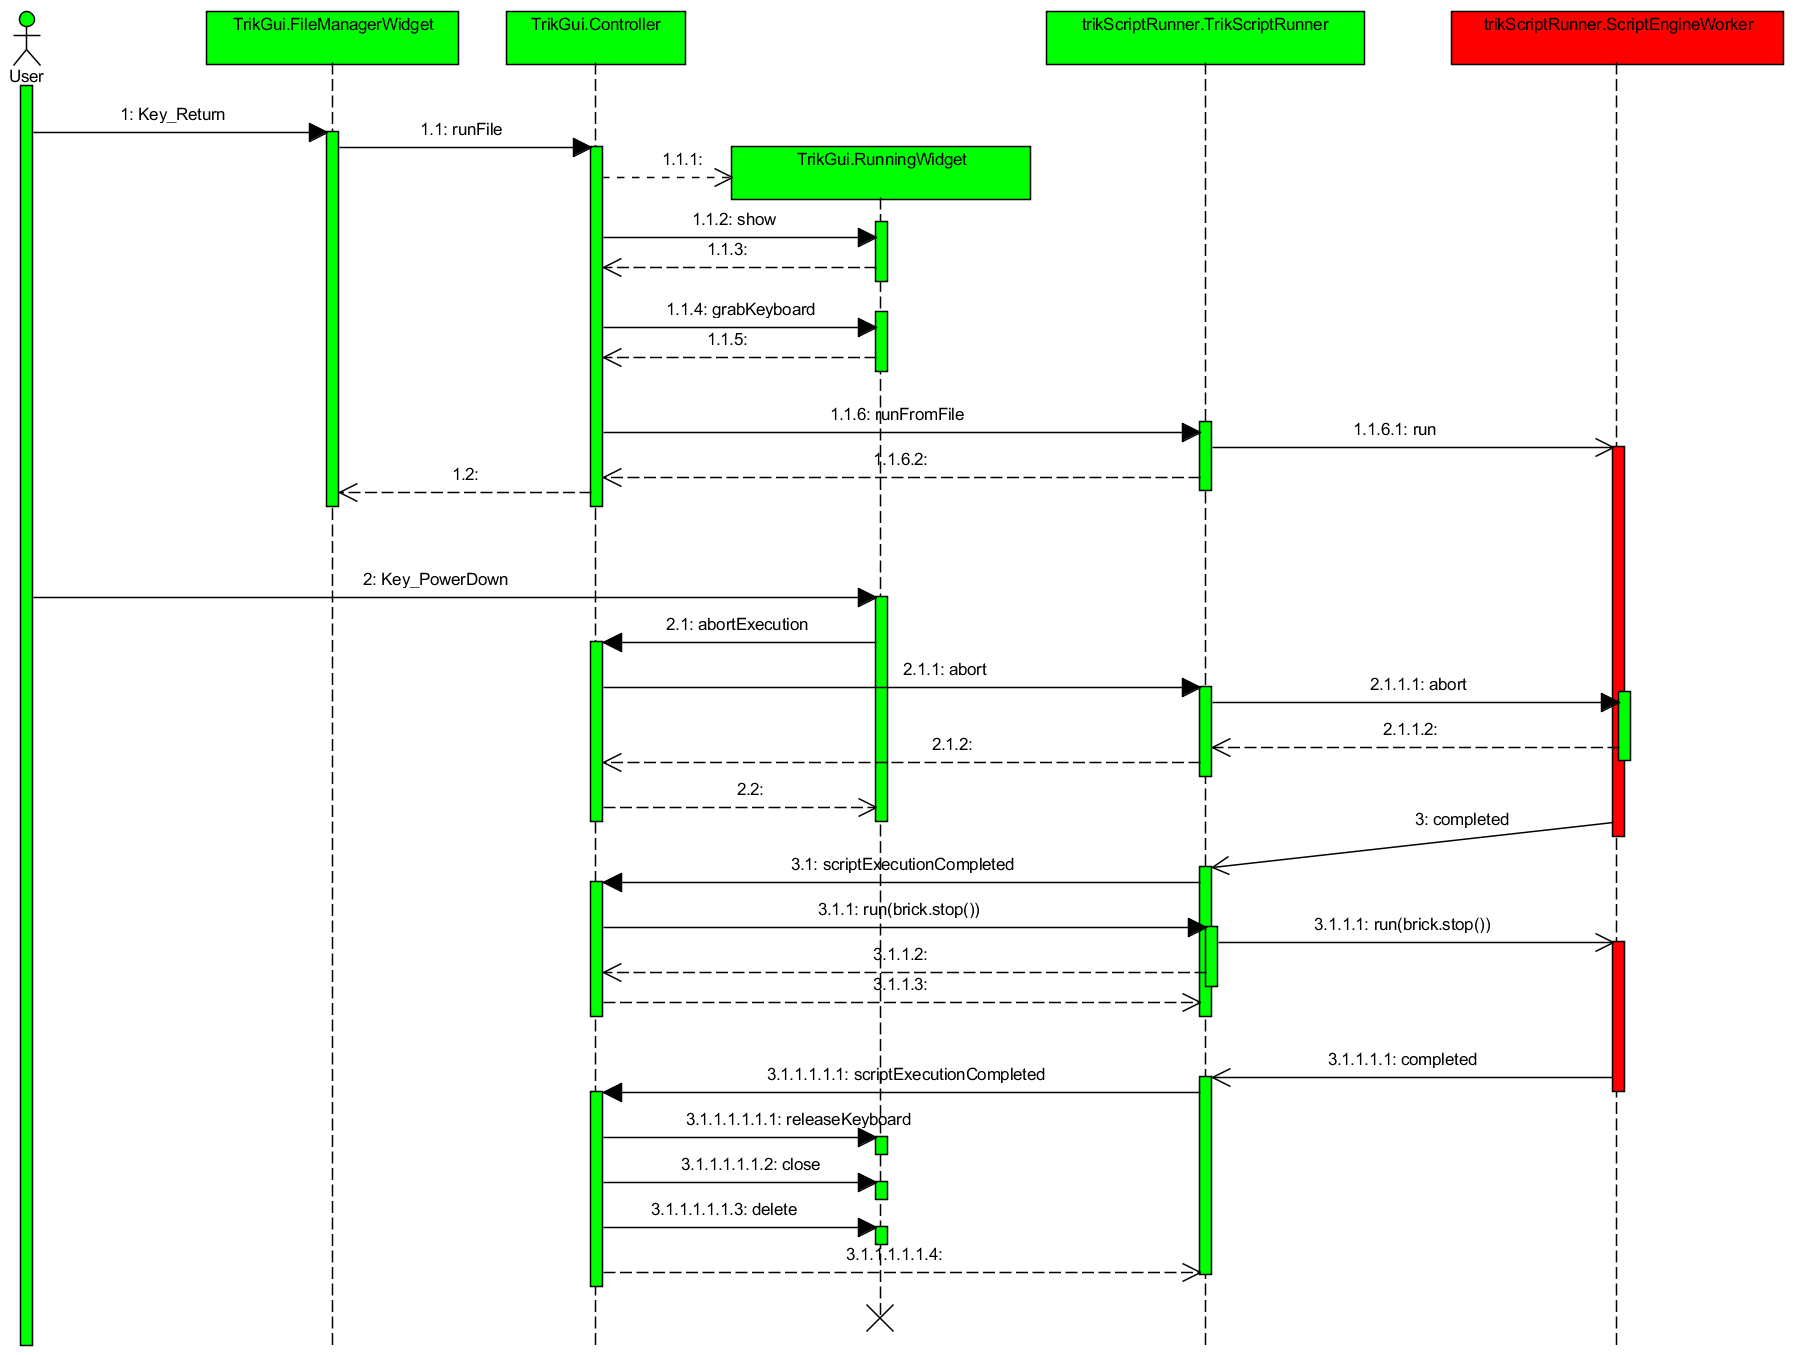
\includegraphics[width=\textwidth]{sequenceDiagramExample3.png}
\end{center}

Это исполнение скрипта на роботе прямо с контроллера. Пользователь выбирает нужный скрипт в меню на экране робота, жмёт <<return>>, после этого инициализируется виджет, отображающий работу скрипта, скрипт запускается в отдельном потоке. Пользователь хочет прервать работу до её естественного окончания, он жмёт на <<powerDown>>, это посылает команду <<abort>> в поток со скриптом, он выполняет согласованную остановку и шлёт обратно <<completed>>. После этого запускается скрипт остановки робота, как в предыдущем примере. Как только он заканчивается, деинициализируем виджет исполнения скрипта и ждём следующие команды. Здесь тоже цветом выделен отдельный поток.

Все три примера взяты из проекта TrikStudio (\footnote{\url{https://github.com/trikset/trik-studio}}), где они показали себя как очень полезные для отладки и вообще понимания того, что происходит.

\subsection{Подробности синтаксиса}

На диаграмме также можно отобразить создание и удаление объекта:

\begin{center}
    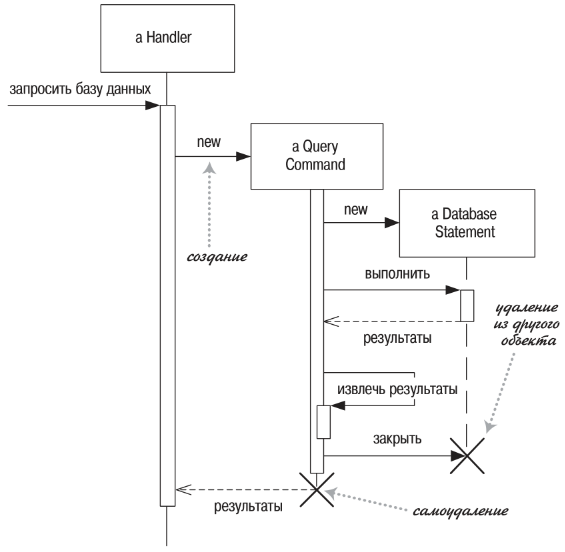
\includegraphics[width=0.5\textwidth]{sequenceDiagramCreationAndDeletion.png}
    \attribution{М. Фаулер, UML. Основы}
\end{center}

Создание означает, как правило, вызов конструктора, удаление более хитро --- либо это вызов деструктора, либо то место, где объект становится больше не нужен и его может собрать сборщик мусора. Создание инициирует другой объект, удаление --- либо сообщением от другого объекта, либо <<самоубийство>> в конце линии активации.

Все средства, описанные выше, позволяют задать только один конкретный сценарий взаимодействия, и обычно диаграммы последовательностей именно для этого и используются. Но если очень надо, можно попытаться отобразить целый алгоритм, с ветвлениями и циклами, с помощью фреймов. Например, псевдокод

\begin{minted}{text}
    foreach (lineitem)
        if (product.value > $10K)
            careful.dispatch
        else
            regular.dispatch
        end if
    end for
    if (needsConfirmation) 
        messenger.confirm
\end{minted}

на диаграмме может выглядеть как

\begin{center}
    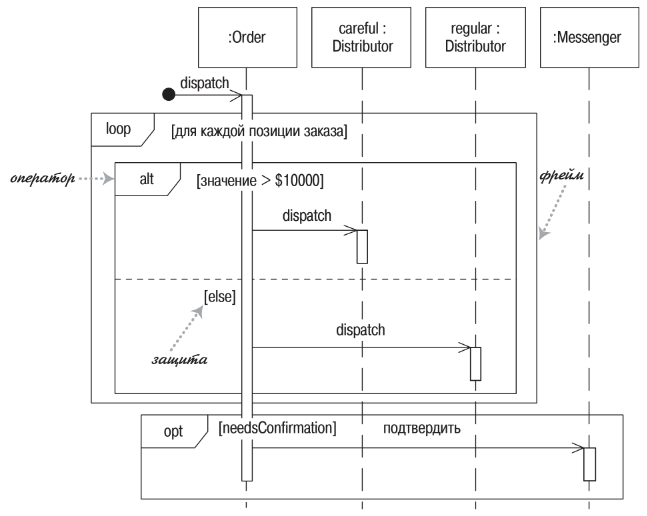
\includegraphics[width=0.6\textwidth]{sequenceDiagramFrames.png}
    \attribution{М. Фаулер, UML. Основы}
\end{center}

Фрейм ограничивает участок взаимодействия и позволяет исполнять его в цикле (фрейм <<loop>>), исполнять разные действия в зависимости от условия (фрейм <<alt>>, который играет роль if или switch/case, поскольку может иметь несколько разделов со взаимоисключающими условиями), просто исполнять или нет в зависимости от условия (фрейм <<opt>>).

Вообще фреймы сильно ухудшают читабельность диаграммы, а для визуализации алгоритмов есть средства получше --- диаграммы активностей, которые мы уже рассматривали, и диаграммы обзора взаимодействия, которые мы слегка рассмотрим дальше. Так что фреймы --- очень ситуационная штука.

\section{Коммуникационные диаграммы}

Коммуникационные диаграммы --- это по сути те же диаграммы последовательностей, только <<с высоты птичьего полёта>>. Они так же применяются для визуализации взаимодействия между объектами, так же подходят только для визуализации одного сценария взаимодействия и так же показывают последовательность обмена сообщениями:

\begin{center}
    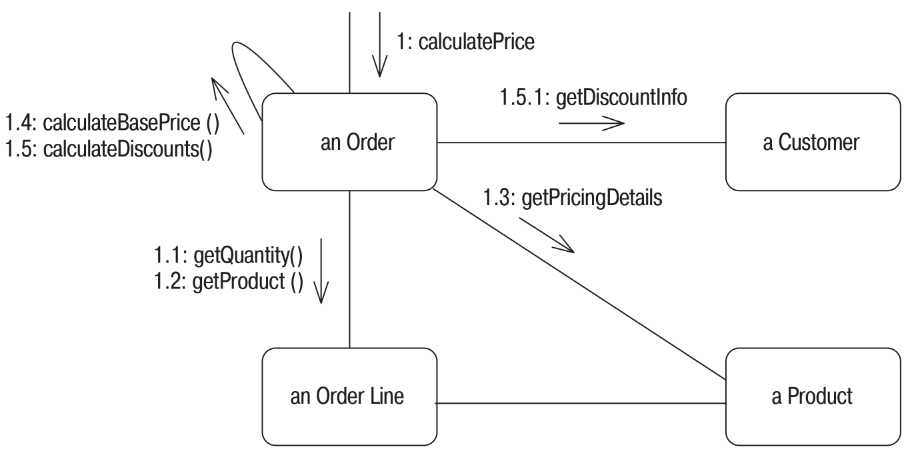
\includegraphics[width=0.6\textwidth]{communicationDiagram.png}
    \attribution{М. Фаулер, UML. Основы}
\end{center}

Однако на диаграммах последовательностей поведение объектов рисуется снизу вверх, то есть, условно, по оси X откладываются объекты, по оси Y --- время. На коммуникационных диаграммах объекты размещаются на двумерной плоскости, а порядок взаимодействия определяется числоввыми индексами на стрелках. Это основное преимущество и основной недостаток таких диаграмм --- они гораздо компактнее диаграмм последовательностей, но порядок действий во времени на них не очевиден.

Вот более содержательный пример, диаграмма коммуникаций для онлайн-магазина книг:

\begin{center}
    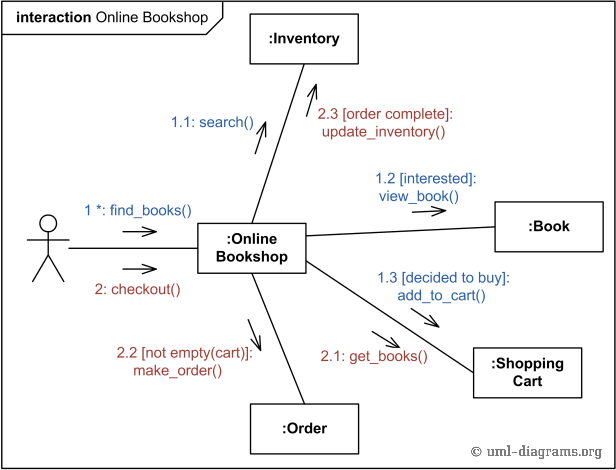
\includegraphics[width=0.6\textwidth]{communicationDiagramExample.png}
    \attribution{http://www.uml-diagrams.org/}
\end{center}

Сначала пользователь делает запрос find\_books(), который обрабатывается объектом типа Online Bookshop (до двоеточия пишется имя объекта, если оно важно, после --- имя типа, если оно важно). Вызов find\_books() приводит к вызову search(), view\_book() и add\_to\_cart() в именно такой последовательности. Обратите внимание на нумерацию запросов: 1.1 означает, что это первый вызов внутри вызова 1, 1.3 --- третий вызов внутри вызова 1. Дальше пользователь выполняет запрос checkout(), который обрабатывается с помощью ещё двух вызовов.

\section{Диаграммы составных структур}

Диаграммы составных структур предназначены больше для проектирования аппаратного обеспечения, которое состоит из стандартизованных блоков, соединённых стандартными интерфейсами. По сути, диаграммы представляют собой продвинутые диаграммы компонентов --- тут тоже рисуются крупные блоки, из которых состоит система, интерфейсы блоков, порты, связи. Однако же если диаграммы компонентов --- это диаграммы, показывающие структуру времени компиляции, то на диаграммах составных структур внутри объемлющей компоненты не другие компоненты, а \textit{роли}. Разница в том, что роль --- это что-то вроде объекта, на диаграмме может быть несколько ролей одного типа, которые по-разному связаны друг с другом и делают разную работу. Так же, как объекты, роли имеют тип. В работающей системе роль может играть любой компонент правильного типа. Вот небольшой пример диаграммы:

\begin{center}
    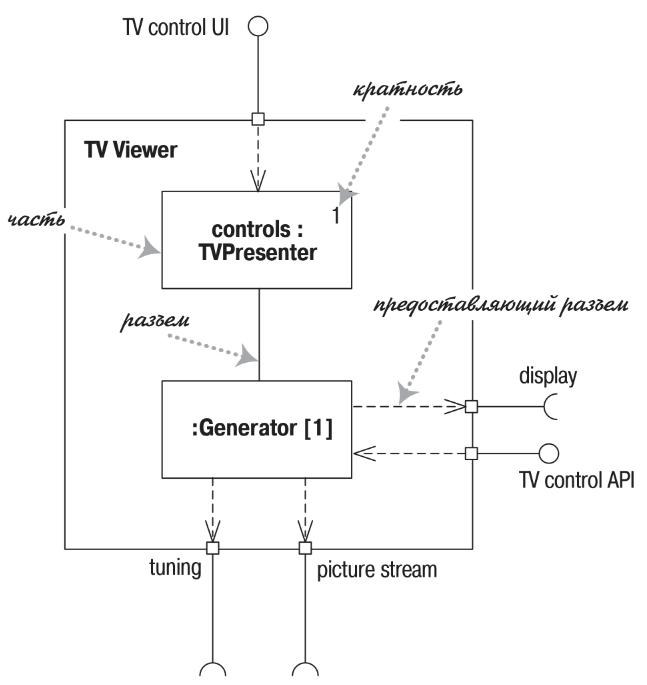
\includegraphics[width=0.5\textwidth]{compositeStructureDiagram.png}
    \attribution{М. Фаулер, UML. Основы}
\end{center}

Тут controls и :Generator --- это роли, в качестве controls может выступать любой компонент, реализующий интерфейс TVPresenter. \verb|[1]| --- это кратность компонента (и TVPresenter, и Generator в системе только один). Порты, интерфейсы и связи тут в целом такие же, как на диаграмме компонентов (только что связи называются ``разьёмами'').

Интерфейсы компонентов можно описывать как в шарово-гнездовой нотации, так и внутри символа компонента:

\begin{center}
    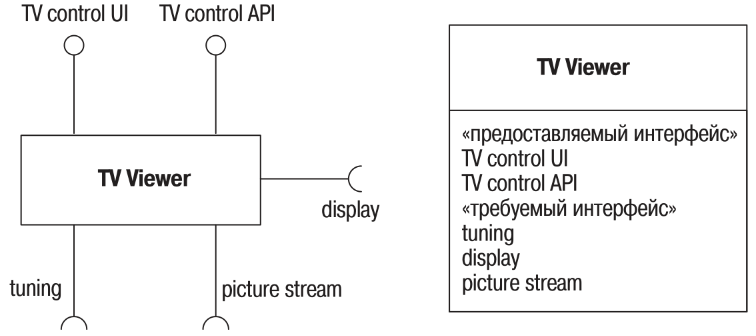
\includegraphics[width=0.6\textwidth]{compositeStructureElement.png}
    \attribution{М. Фаулер, UML. Основы}
\end{center}

Вот пример побольше, с \url{http://www.uml-diagrams.org/}:

\begin{center}
    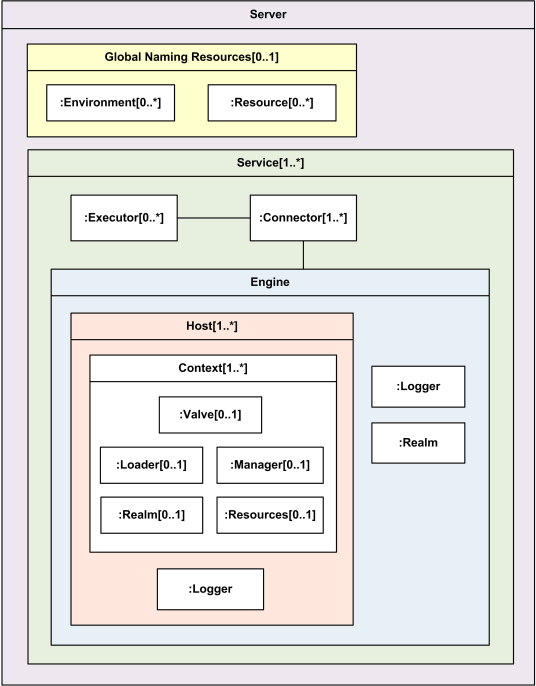
\includegraphics[width=0.6\textwidth]{compositeStructureExample.png}
    \attribution{http://www.uml-diagrams.org/}
\end{center}

Выделение цветом в стандарте не прописано, но он его и не запрещает, поэтому этим часто пользуются (особенно на диаграмме компонентов и на диаграмме составных структур, где цвет удобен для визуализации иерархичности).

\section{Диаграммы коопераций}

Диаграммы коопераций --- это что-то среднее между диаграммами объектов и диаграммами классов. Вместо классов и объектов на них рисуются \textit{роли} --- сущности, на место которых может быть подставлен настоящий объект. Диаграммы показывают взаимодействие ролей в рамках одного сценария использования, например:

\begin{center}
    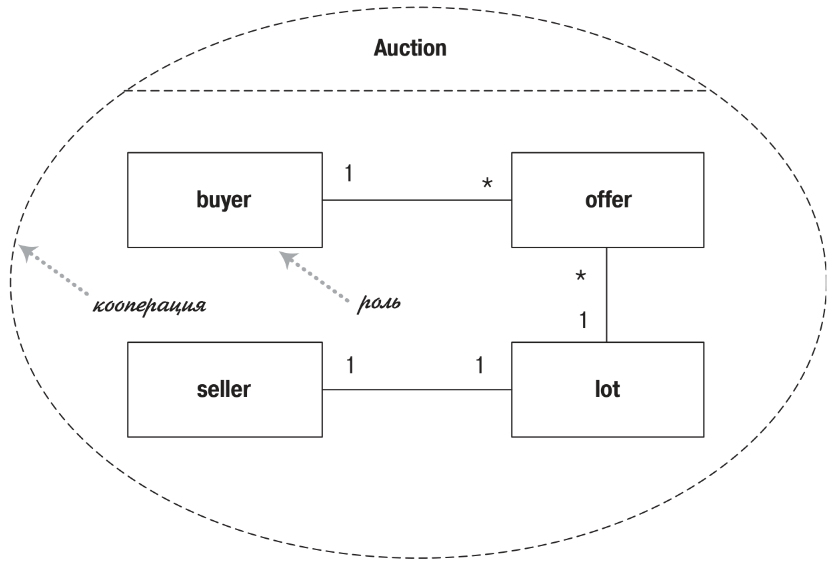
\includegraphics[width=0.7\textwidth]{cooperationDiagram.png}
    \attribution{М. Фаулер, UML. Основы}
\end{center}

Либо, что то же самое,

\begin{center}
    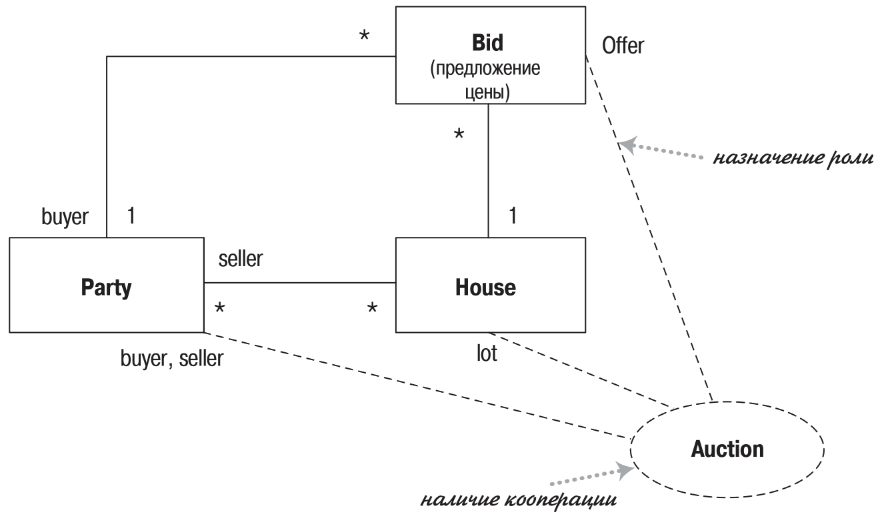
\includegraphics[width=0.7\textwidth]{cooperationAlternateNotation.png}
    \attribution{М. Фаулер, UML. Основы}
\end{center}

Здесь показана кооперация в рамках сценария использования <<Аукцион>>. Есть роли <<покупатель>>, <<продавец>>, которые могут взаимодействовать посредством лотов и предложений. Второй стиль рисования такой диаграммы больше похож на диаграмму классов, есть класс <<сторона>>, исполняющий роли <<покупатель>> и <<продавец>> в рамках данного взаимодействия.

Нужны такие диаграммы, чтобы проиллюстрировать конкретный сценарий использования системы, либо чтобы сосредоточиться на анализе конкретного сценария. Эти диаграммы предоставляют простую структурную точку зрения на объекты, и могут дополняться диаграммами последовательностей для иллюстрации ещё и временных аспектов:

\begin{center}
    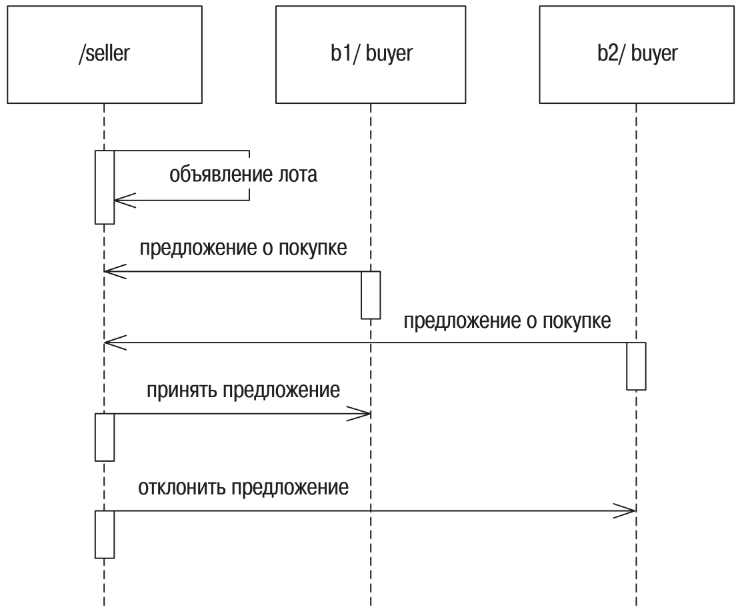
\includegraphics[width=0.7\textwidth]{cooperationSequenceDiagram.png}
    \attribution{М. Фаулер, UML. Основы}
\end{center}

На диаграммах последовательностей в таких случаях пишут имя объекта <</>> имя роли, которую этот объект играет в системе. Тут, например, видно, что покупателя в данном взаимодействии два.

\section{Временные диаграммы}

Временные диаграммы создавались прежде всего для инженеров-электронщиков или для людей, проектирующих системы реального времени. Они нужны, чтобы визуализировать последовательности событий с чёткими временными ограничениями. Есть два варианта синтаксиса:

\begin{center}
    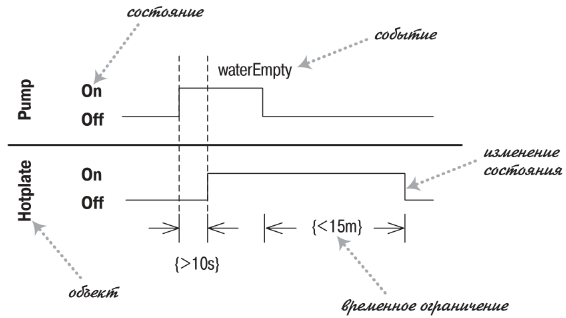
\includegraphics[width=0.6\textwidth]{timingDiagrams.png}
    \attribution{М. Фаулер, UML. Основы}
\end{center}

и

\begin{center}
    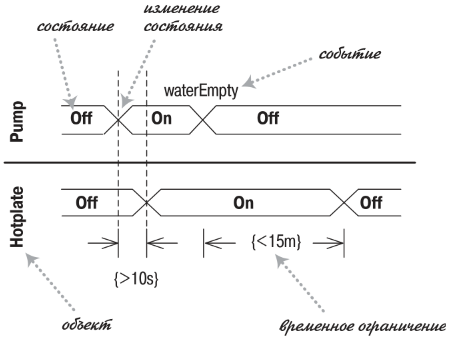
\includegraphics[width=0.6\textwidth]{timingDiagramsAlternate.png}
    \attribution{М. Фаулер, UML. Основы}
\end{center}

В обоих случаях рисуется временная шкала (время идёт слева направо), на ней вертикально располагаются объекты, которые могут находиться в некоторых состояниях. Первый вариант показывает переключение состояния как скачок линии, второй --- как пересечение линий с именем состояния внутри. Второй вариант удобнее, если состояний много, первый вариант нагляднее. Помимо состояний указываются и временные ограничения, в фигурных скобках, как принято в UML для ограничений.

Вот более солидный пример, для запроса браузера:

\begin{center}
    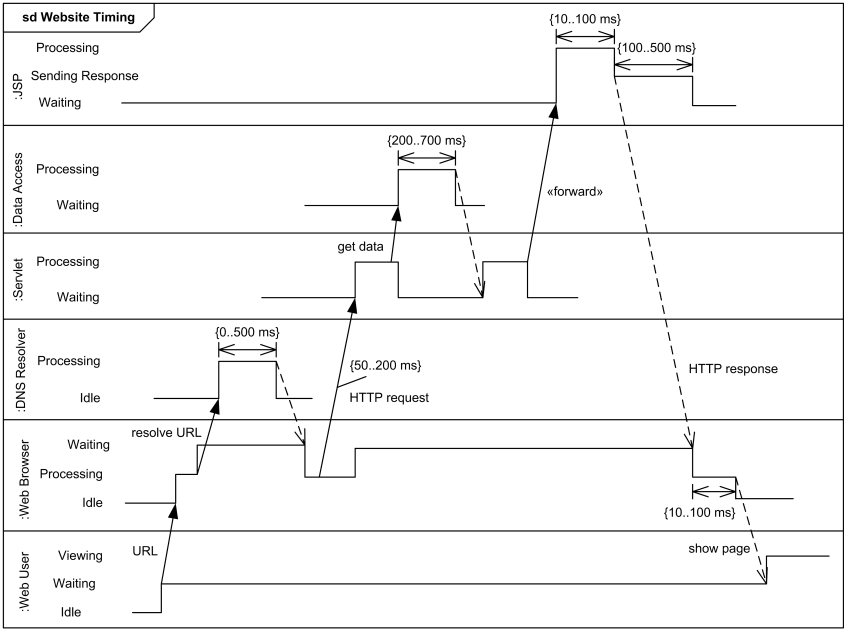
\includegraphics[width=0.9\textwidth]{timingDiagramExample.png}
    \attribution{http://www.uml-diagrams.org/}
\end{center}

Видно, что диаграмма позволяет отразить последовательность событий столь же наглядно, как диаграмма последовательностей, но ещё и наглядно показывает временные ограничения, и гораздо нагляднее в плане последовательности изменений внутреннего состояния объектов.

\section{Диаграммы обзора взаимодействия}

Диаграммы обзора взаимодействия --- это на самом деле не более чем совмещённые на одной диаграмме элементы диаграммы последовательностей и диаграммы активностей. Выглядят они так:

\begin{center}
    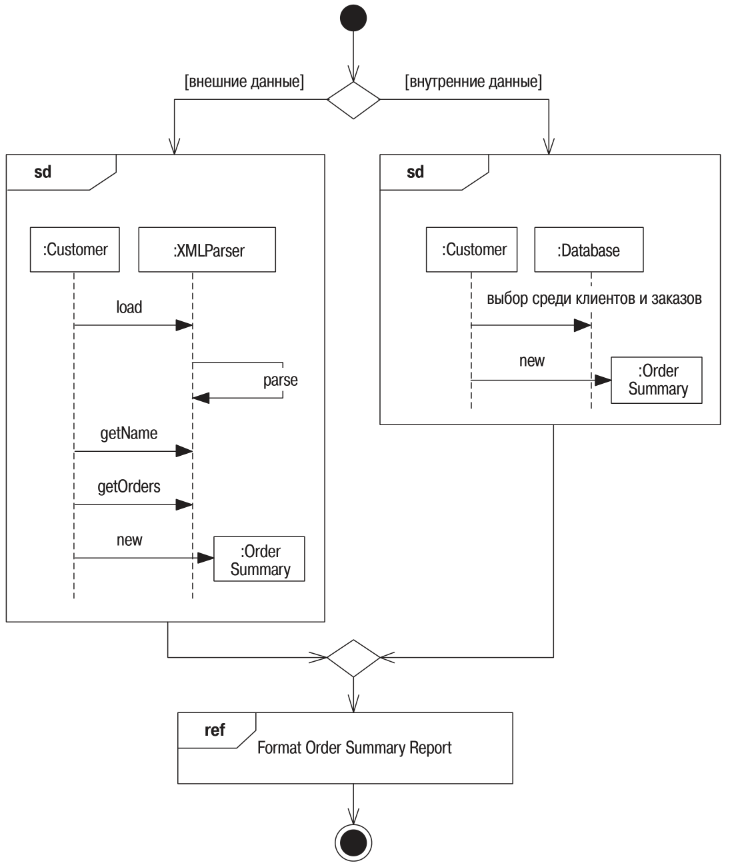
\includegraphics[width=0.7\textwidth]{interactionOverviewDiagrams.png}
    \attribution{М. Фаулер, UML. Основы}
\end{center}

Видно, что активность из диаграммы активностей может быть представлена в виде последовательности действий на диаграмме последовательностей. Применяются такие диаграммы, когда есть сложный алгоритм и нужна диаграмма последовательностей, которая бы его визуализировала, но имеется куча ветвлений и циклов. На диаграммах последовательностей есть фреймы, но для сколько-нибудь сложных алгоритмов они быстро сделают диаграмму нечитаемой --- тут-то диаграммы обзора взаимодействия и пригодятся. 

Вот более содержательный пример, валидация комментариев на сайте:

\begin{center}
    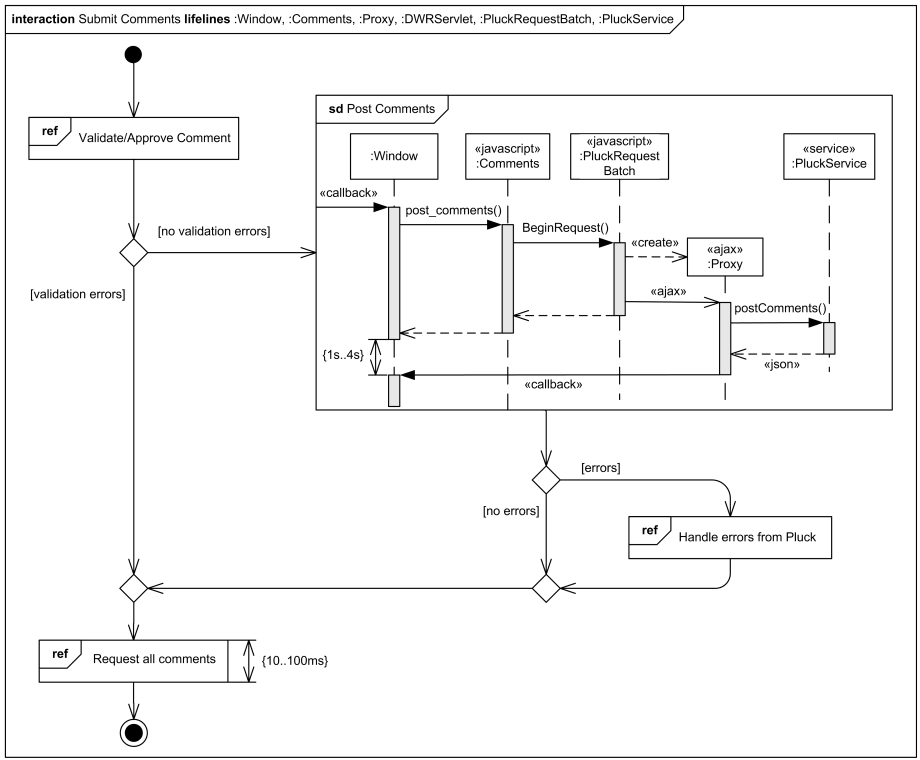
\includegraphics[width=0.9\textwidth]{interactionOverviewExample.png}
    \attribution{http://www.uml-diagrams.org/}
\end{center}

Как видно, на таких диаграммах тоже могут указываться временные ограничения.

\section{Диаграммы потоков данных}

На этом рассмотрение диаграмм UML закончилось. Но есть ещё полезные диаграммы, часто используемые сейчас при моделировании поведения программ, которые в UML не входят и даже не имеют там аналогов. 

Первая такая диаграмма, пожалуй, самая популярная и самая древняя из них --- это диаграмма потоков данных (Data Flow Diagram):

\begin{center}
    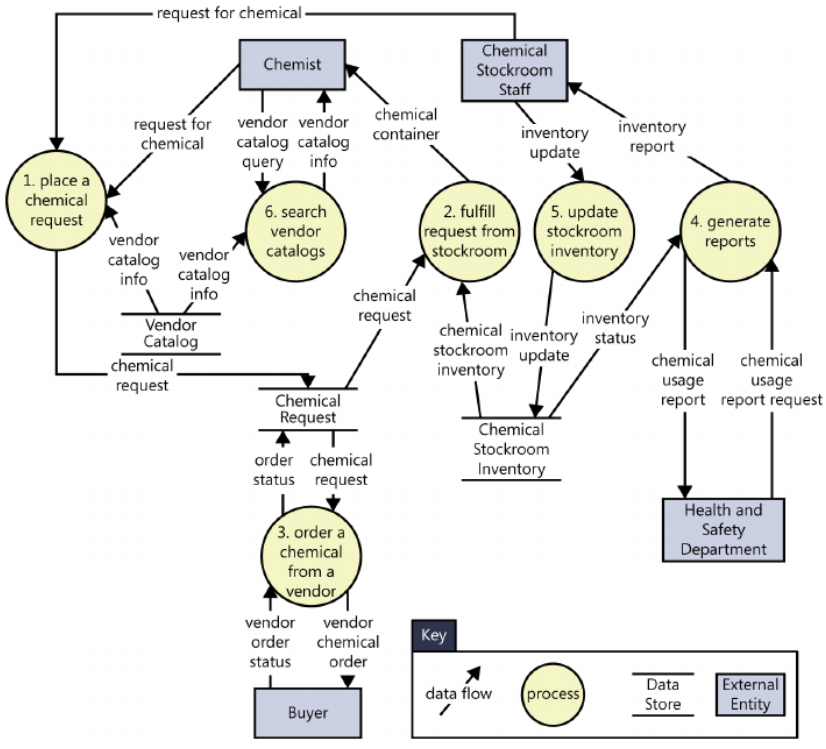
\includegraphics[width=0.8\textwidth]{dfd.png}
\end{center}

Синтаксис очень прост, есть один вид стрелок, который показывает поток данных, и три вида сущностей, между которыми, собственно, ходят данные:

\begin{itemize}
    \item процесс --- то, что может как-то преобразовывать данные внутри проектируемой системы, рисуется кружком;
    \item внешняя сущность --- то, что поставляет или потребляет данные, рисуется прямоугольником;
    \item хранилище --- то, где данные могут лежать, куда их можно поместить и забрать при необходимости, рисуется двумя горизонтальными линиями.
\end{itemize}

Такие диаграммы полезны как первый наборосок архитектуры системы (например, когда есть бизнес-процесс, где данные уже как-то ходят) или как иллюстрация к уже созданной системе. Потоки данных между функциональными блоками обычно интуитивно понятны и вместе с тем довольно сложны, так что диаграммы потоков данных могут сообщить много информации человеку, который начинает знакомиться с системой.

\section{Диаграммы IDEF0}

Контекстные диаграммы IDEF0 в этом курсе уже упоминались, их дальнейшая детализация --- диаграммы, описывающие декомпозицию системы и связи между её частями (которые, в свою очередь, тоже могут быть декомпозированы и раскрыты на отдельных диаграммах). Вот пример диаграммы IDEF0:

\begin{center}
    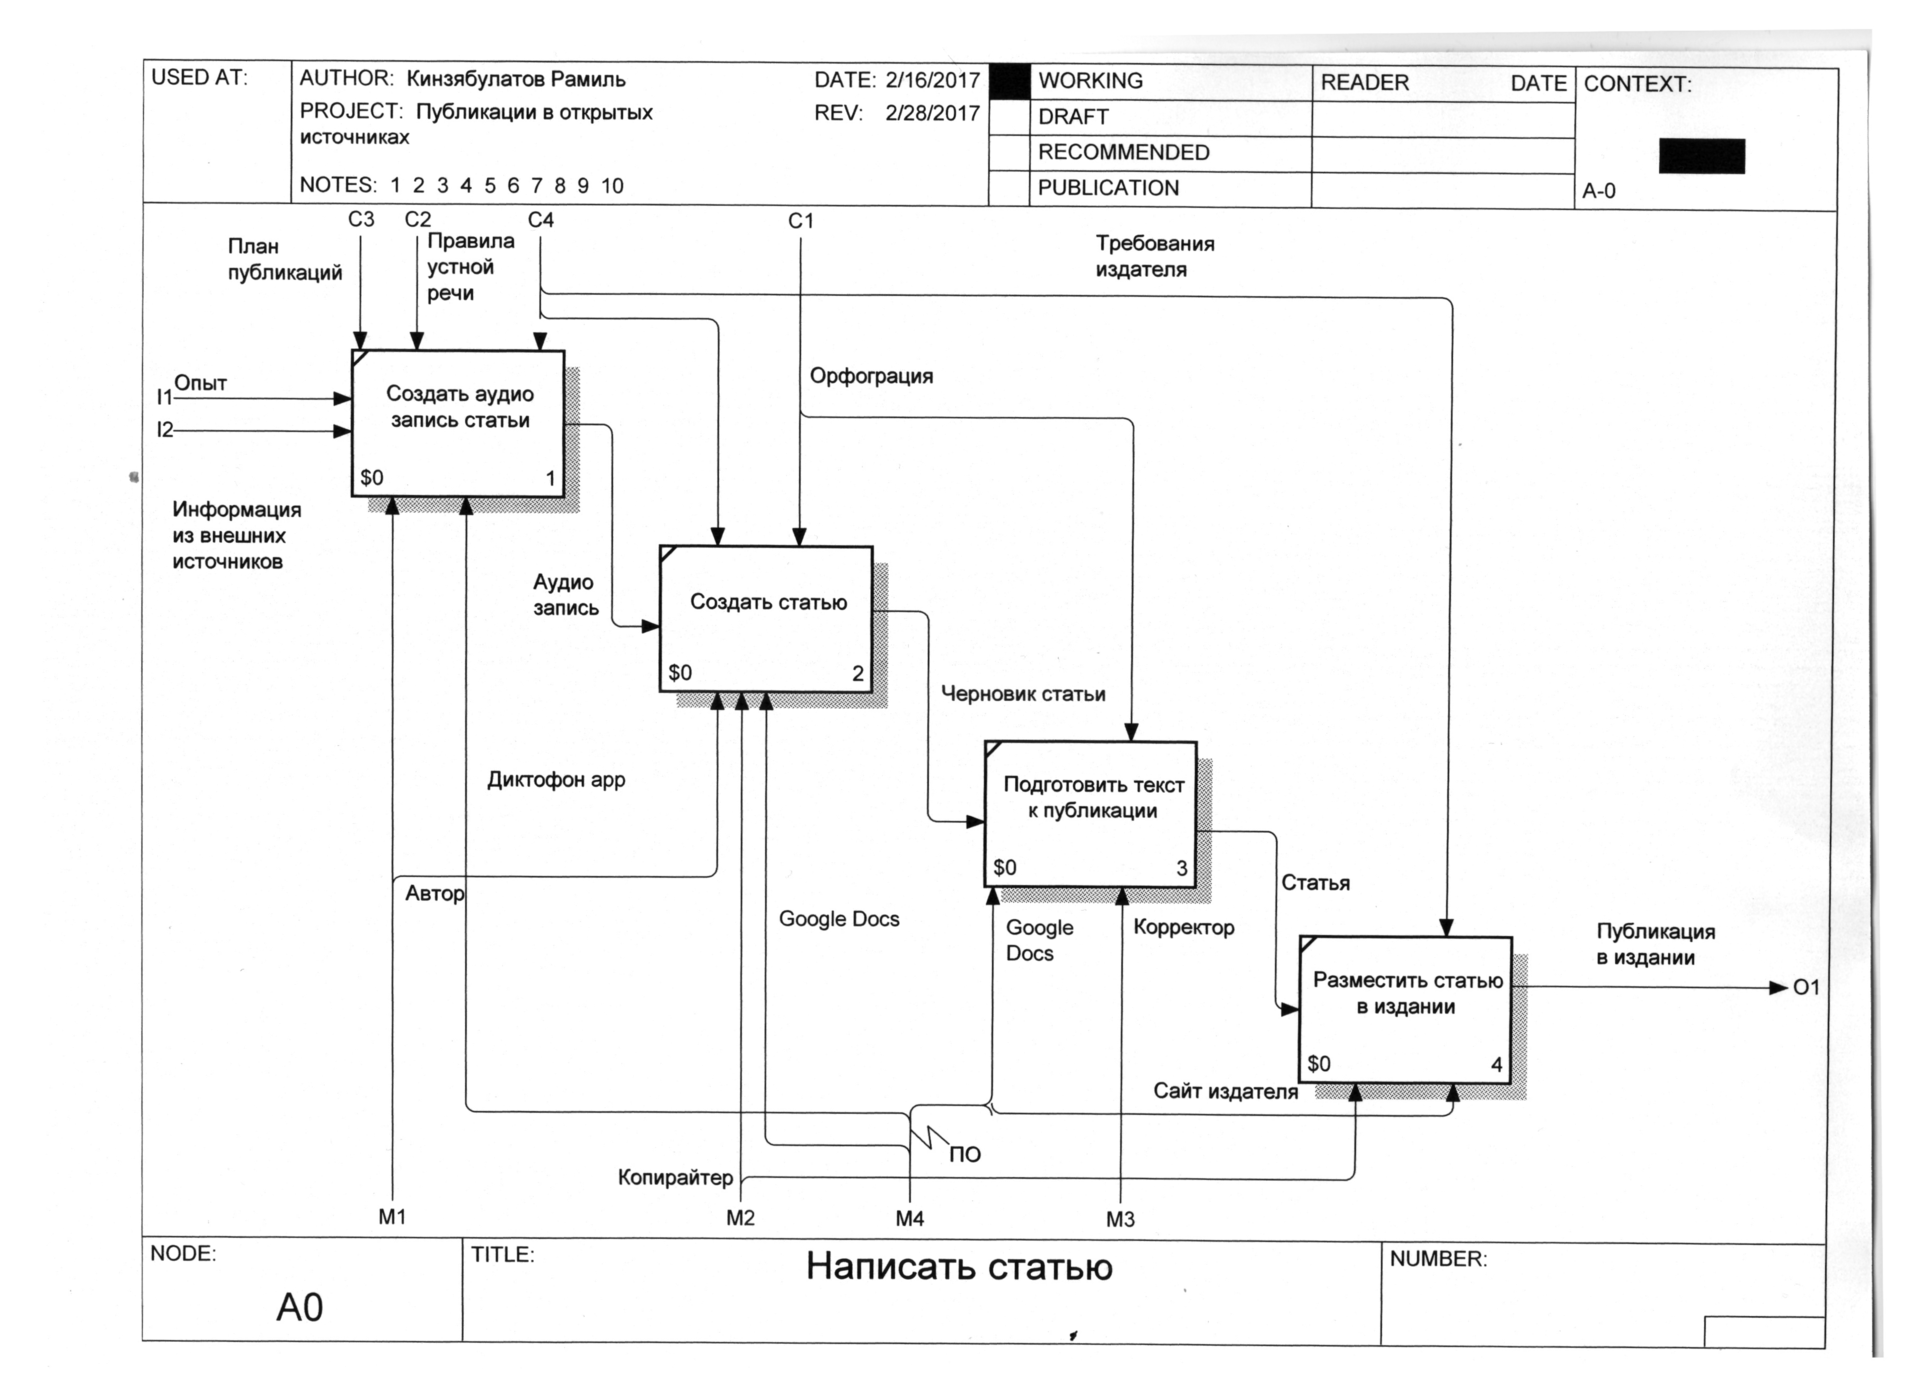
\includegraphics[width=\textwidth]{idef0.png}
    \attribution{https://habrahabr.ru/post/322832/}
\end{center}

Диаграмма состоит из блоков (у каждого из них есть имя и однозначно идентифицирующий его номер) и стрелок. Стрелки, входящие в блок слева --- материалы, которые блок перерабатывает в результаты (стрелки, выходящие справа). Сверху входят стрелки-управления --- то, что регламентирует работу блока и как-то управляет им. Снизу входят стрелки-механизмы (или ресурсы) --- это то, что блок непосредственно не перерабатывает, но необходимо блоку для работы. Например, блок может быть автозаводом, он перерабатывает запчасти в автомобили, как механизмы он использует станки и рабочих, как управление --- государственные и отраслевые стандарты, заказы от дилеров.

Над стрелками пишется, что из себя представляет эта стрелка, стрелки могут ветвиться (что может означать просто разделение ветки или детализацию --- тогда над отделившимися ветками пишутся уточнения надписи, которая была на исходной ветке) и сходиться в одну. Все ветки, входящие извне или исходящие с диаграммы, должны входить в блок или выходить из блока на диаграмме уровнем выше, и так далее до контекстной диаграммы. При этом используется однозначная схема именования стрелок.

Такие диаграммы чаще используются в анализе бизнес-процессов; в разработке собственно ПО чаще применяются всё-таки диаграммы UML (диаграммы компонентов и диаграммы составных структур прекрасно заменяют IDEF0 в большинстве случаев). Тем не менее, аналитики IDEF0 любят и часто передают архитекторам как результаты своей работы, поэтому владеть IDEF0 архитекторам приходится.

\section{Сети Петри}

Сети Петри, в отличие от всего выше рассмотренного --- это не просто визуальная нотация, а математический формализм, который просто обзавёлся визуальной нотацией потому, что это удобно. Сети Петри --- ценный метод анализа параллельных программ, а поскольку подавляющее большинство современных систем так или иначе параллельны, сети Петри могут быть довольно полезны на практике (хотя в действительности IT-компаний сети Петри автор пока не встречал).

Итак, сеть Петри --- это граф из мест, переходов и токенов, которые могут находиться в местах и прыгать через переходы. Простой пример сети Петри (для задачи производителя-потребителя):

\begin{center}
    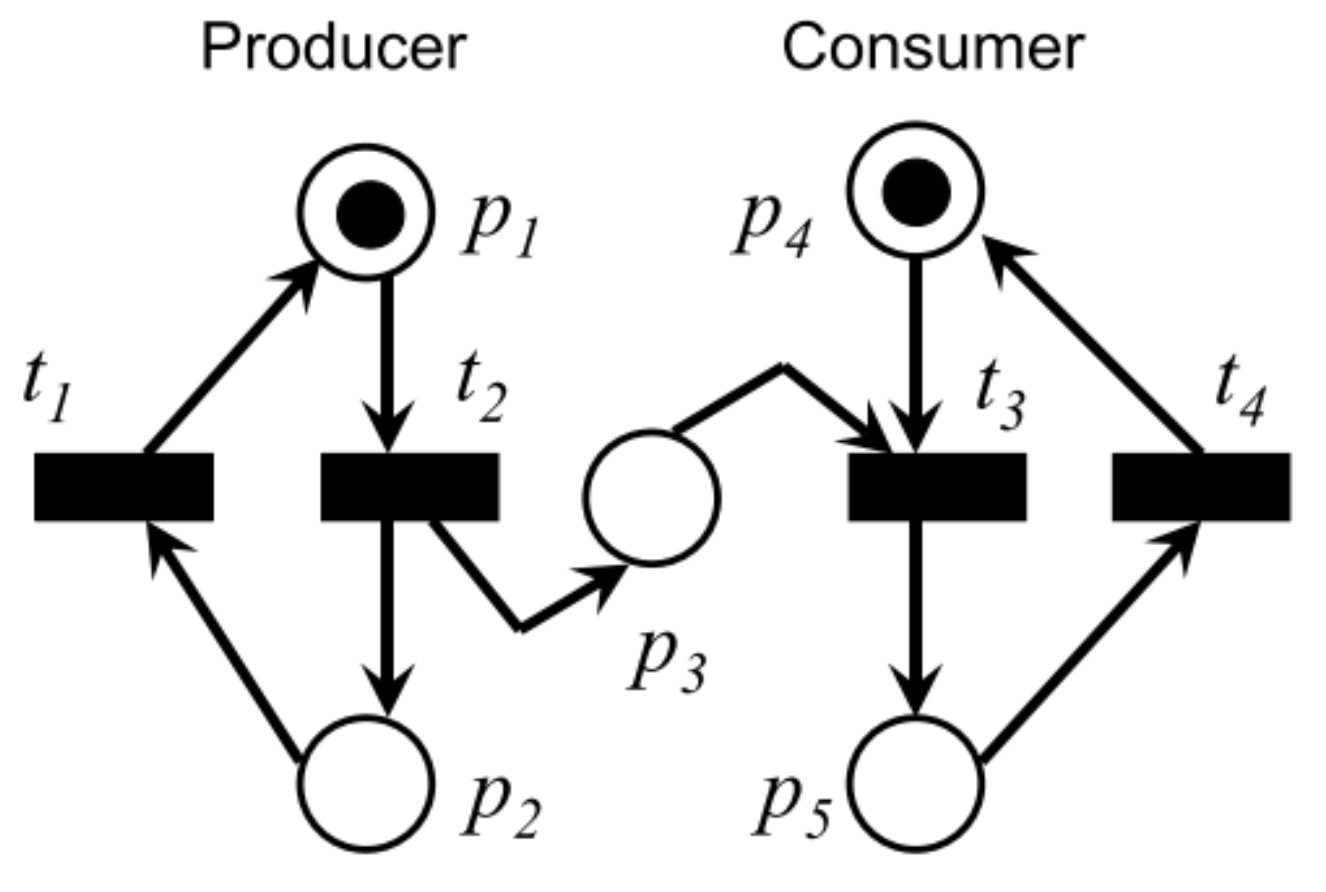
\includegraphics[width=0.4\textwidth]{petri.png}
\end{center}

Места рисуются кругами, переходы --- закрашенными прямоугольниками, а токены --- закрашенными кругами внутри мест. Токенов может быть много, как во всей диаграмме, так и в каждом месте. У диаграмм есть семантика --- переход может \textit{сработать}, если во всех его входных местах есть хоть один токен, и тогда он забирает по одному токену из каждого входного места и помещает по одному токену в каждое выходное место. 

Так что в нашем примере готов к срабатыванию только переход $t_2$ (для перехода $t_3$ один токен есть, но ему два надо, в месте $p_3$ токена нету). Когда переход $t_2$ сработает, из места $p_1$ токен исчезнет, зато появится по токену в местах $p_2$ и $p_3$. И тогда уже $t_3$ сможет сработать, но одновременно с ним может сработать и $t_1$. Считается, что из готовых переходов срабатывающий выбирается случайно, другая точка зрения на это --- что все переходы срабатывают и не срабатывают одновременно, порождая из одного состояния множество состояний (как в недетерминированных автоматах). Теперь должно быть понятно, почему сеть из примера иллюстрирует задачу производителя-потребителя: $p_3$ --- это буфер с данными, Producer бегает в цикле, производит новые данные и кладёт их в буфер, Consumer, если буфер не пуст, бегает в цикле и забирает из буфера данные, параллельно с Producer. Токены в местах $p_1$ и $p_2$ симулируют текущую исполняемую инструкцию производителя, в местах $p_4$ и $p_5$ --- текущую исполняемую инструкцию потребителя, токены в месте $p_3$ --- данные в буфере (их может накопиться сколь угодно много, если производитель работает быстрее).

Однако диаграмма в случае с сетями Петри --- это только вершина айсберга. Формально, сеть Петри --- это:

\begin{itemize}
    \item тройка $(P, T, \phi)$, где
    \begin{itemize}
        \item $P$ --- множество мест;
        \item $T$ --- множество переходов;
        \item $\phi$ --- функция потока: $\phi : (P \times T) \cup (T \times P) \rightarrow \mathbb{N}$ --- определяет связи между местами и переходами ($\mathbb{N}$ --- множество натуральных чисел, число показывает, сколько токенов переход забирает, и сколько кладёт в место);
    \end{itemize}
    \item маркировка: $\mu : P \rightarrow \mathbb{N}$ --- каждому месту сопоставляет количество токенов, которые в нём сейчас находятся;
    \item cрабатывание (firing):
    $\mu \xrightarrow{t} \mu’ : \mu’(p) = \mu(p) - \phi(p, t) + \phi(t, p), \forall p \in P$ --- собственно, переклазывает токены при срабатывании перехода.
\end{itemize}

Вот несколько примеров сетей Петри из хорошей, хоть и старой, обзорной статьи Murata Tadao <<Petri nets: Properties, analysis and applications>>:

\begin{center}
    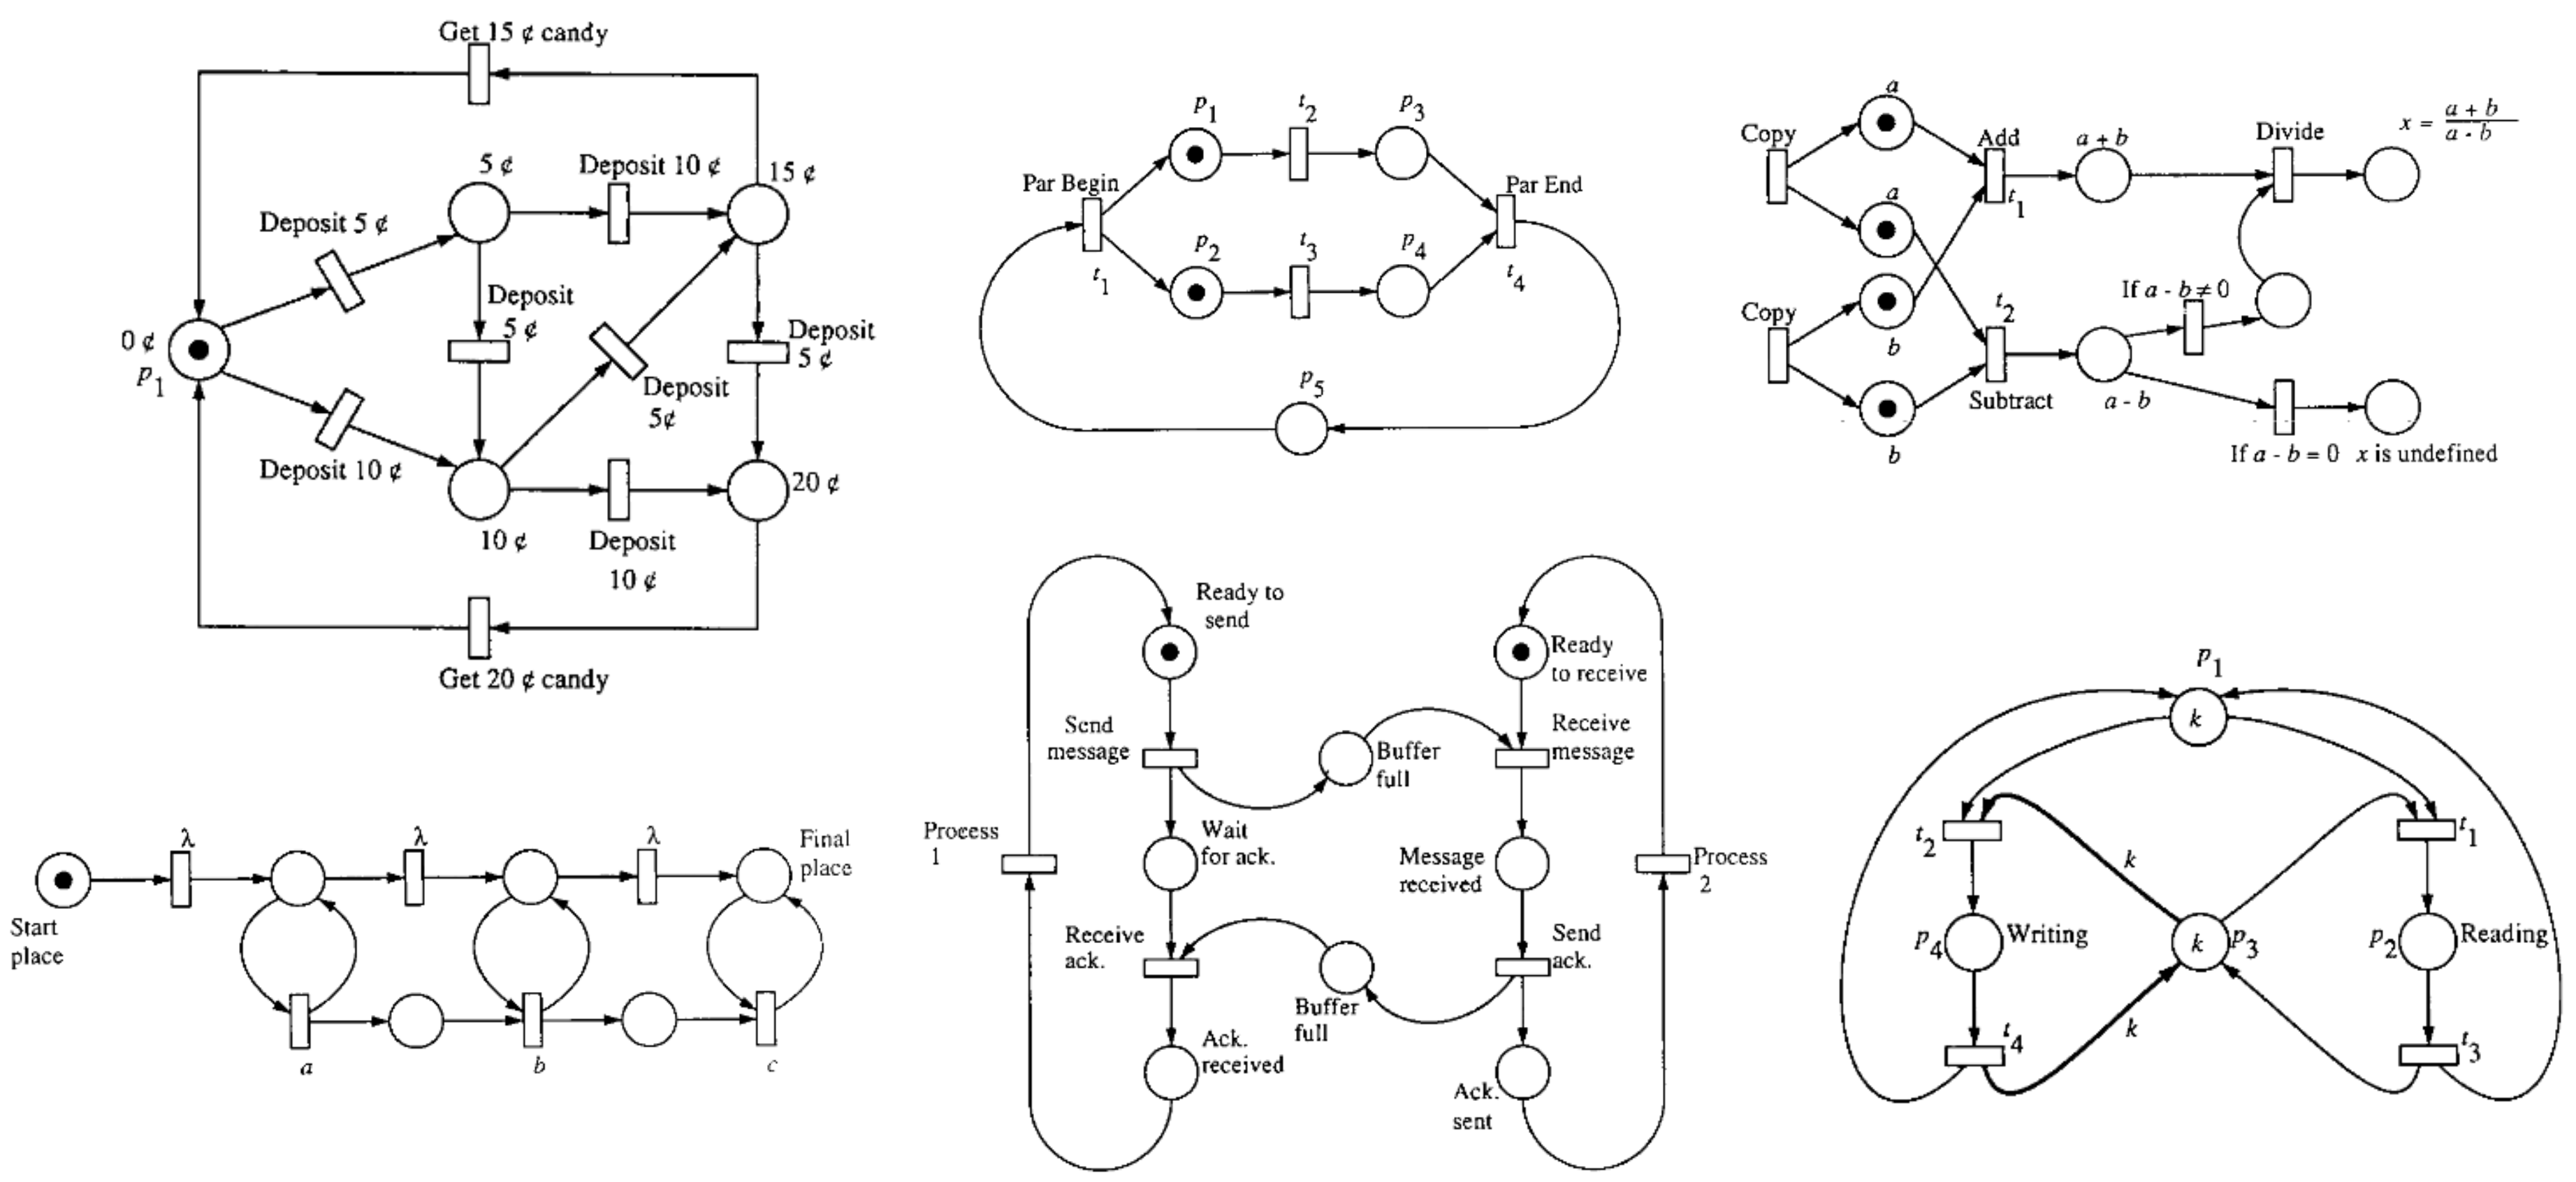
\includegraphics[width=0.95\textwidth]{petriNetExamples.png}
    \attribution{Murata Tadao. Petri nets: Properties, analysis and applications}
\end{center}

Слева вверху, кстати, уже знакомый нам пример торгового автомата, который показывает, что вообще конечные автоматы --- это частный случай сетей Петри (точнее, сеть, у которой каждый переход имеет ровно одно входное и ровно одно выходное место). Второй пример сверху показывает типичный параллельный кусок кода, который сначала разветвляется на два потока, потом потоки соединяются (например, функцией join()). Третий пример сверху показывает моделирование арифметической операции, а заодно и то, что у перехода может вообще не быть входных мест (тогда он просто бесконечно производит токены из ниоткуда). Кстати, может не быть и выходных --- тогда переход <<пожирает>> все токены.

\subsection{Свойства сетей Петри}

Зачем это всё вообще нужно: дело в том, что сети Петри с так определёной семантикой не тьюринг-полны, что, во-первых, означает, что не любая программа может быть точно смоделирована сетью Петри, а во-вторых, и в главных, что некоторые полезные свойства программ оказываются алгоритмически разрешимыми. Вот свойства, которые можно за конечное время доказать или опровергнуть для любой сети Петри:

\begin{itemize}
    \item Поведенческие свойства (доказываемые для сети Петри с конкретной маркировкой, то есть распределением токенов по местам):
    \begin{itemize}
        \item достижимость --- что из заданной маркировки сети можно достичь другой заданной маркировки. Это означает, что можно доказать, что программа в принципе завершится (что невозможно в общем случае) или попадёт в заданное состояние.
        \item Ограниченность --- что количество токенов в любом месте сети никогда не будет больше некоторого наперёд заданного числа, и более сильное свойство, \textit{безопасность} --- что количество токенов в любом месте сети никогда не будет больше 1, какие бы переходы в какой бы последовательности ни срабатывали (в программе никогда не будет переполнения буфера).
        \item Живость --- целый набор свойств, гарантирующий разные степени утверждения <<в программе нет дедлоков и она никогда не зависнет>>. \textit{L0-живость} означает, что сеть <<мертва>>, то есть ни один её переход никогда не сработает; \textit{L1-живость} означает, что каждый переход сети может потенциально сработать, то есть существует такая последовательность срабатываний, когда переход сработает (в программе нет мёртвого кода); \textit{L4-живость} означает, что любой переход может всегда сработать, то есть L1-жив в любой маркировке, достижимой из заданной (программа не может оказаться в состоянии, в которое не сможет вернуться, все состояния всегда достижимы).
        \item <<Реверсабельность>> --- из любого состояния, достижимого из исходного, мы всегда можем попасть в исходное; и более слабое свойство --- <<домашнее состояние>> --- когда из исходного достижимо такое состояние, в которое можно попасть из любого состояния, которое из него достижимо. Реверсабельность в программах означает, что мы всегда можем вернуться к исходному состоянию, что бы мы ни делали, а <<домашнее состояние>> означает, что сначала программа может как-то инициализироваться, выполнять дополнительную установку и т.д., но как только она готова к работе, она, например, показывает стартовый экран, на который мы всегда можем вернуться.
        \item и т.д., есть ещё интересные свойства, которые можно доказывать, см. статью M. Tadao.
    \end{itemize}
    \item Структурные свойства (доказываемые для сети Петри с \textbf{любой} маркировкой):
    \begin{itemize}
        \item структурная живость --- существует хотя бы одна маркировка, при которой сеть L1-жива (нет мёртвого кода);
        \item полная контролируемость --- любая маркировка достижима из любой другой маркировки (что бы мы ни делали с программой, мы всегда можем попасть в любое её состояние за конечное число шагов);
        \item структурная ограниченность --- что при любой конечной начальной маркировке количество токенов в каждом месте не превосходит некоторого наперёд заданного для данной маркировки числа (в программе в принципе невозможны переполнения буфера);
        \item консервативность --- количество токенов в сети константно (программа корректно обрабатывает физические ресурсы, которые нельзя просто раскопировать);
        \item и т.д. и т.п.
    \end{itemize}
\end{itemize}

\subsection{Способы анализа}

Доказывать вышеприведённые свойства для данной сети можно разными способами. Самый алгоритмически эффективный, но вместе с тем самый слабый способ анализа --- это алгебраический. Посмотрим на состояние сети Петри как на вектор длины $|P|$, где на $i$-й позиции будет стоять число токенов в месте $i$. И определим матрицу переходов $M$, где $M_{i, j}$ будет равно количеству токенов, которые $i$-й переход кладёт в $j$-е место ($M_{i, j}$ больше нуля для выходных мест перехода и меньше нуля для входных). Тогда просимулировать состояние сети после нескольких переходов мы можем, прибавив вектор начального состояния к матрице переходов, умноженной на вектор срабатываний (вектор размерностью $|T|$, где на $i$-й позиции стоит число срабатываний перехода $i$). Например:

\begin{center}
    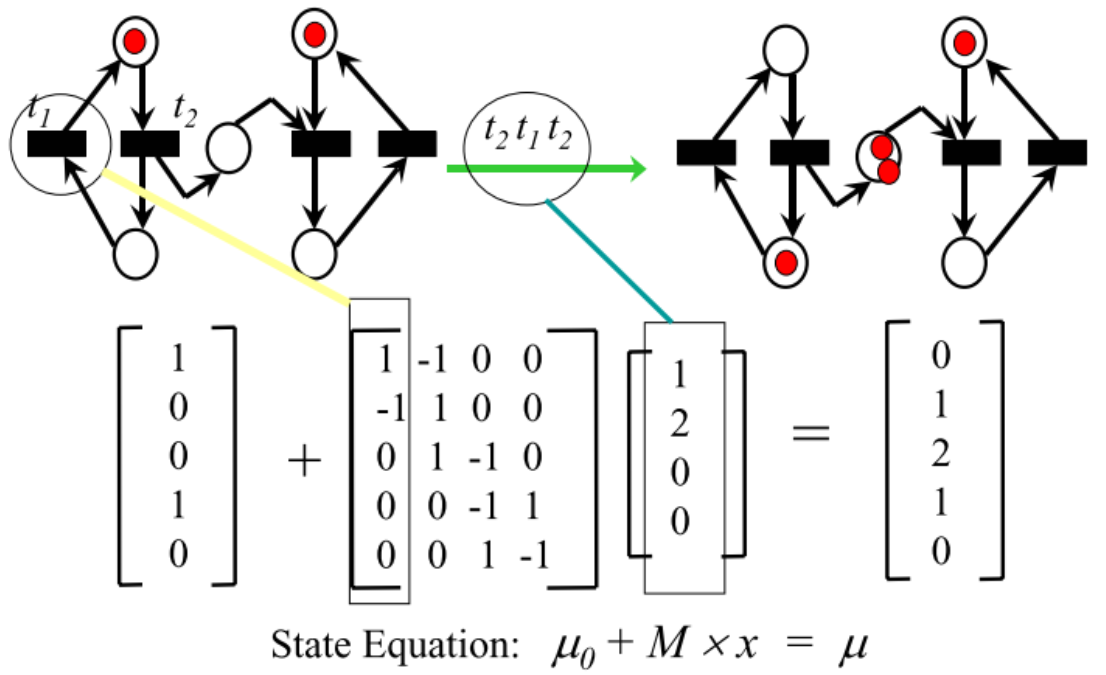
\includegraphics[width=0.7\textwidth]{petriAlgebraicAnalysis.png}
\end{center}

Матрицу переходов легко построить по данной сети (и она зависит только от топологии сети), вектор начального состояния легко строится по начальной маркировке (собственно, он и есть начальная маркировка). Желаемое конечное состояние обычно известно, так что мы можем записать уравнение, где неизвестным будет вектор переходов. Если такое уравнение не решается, то конечное состояние точно недостижимо из начального (а решать системы линейных уравнений можно за полиномиальное время). Однако если такое уравнение решается, это, внезапно, ещё ничего не значит. Простой пример:

\begin{center}
    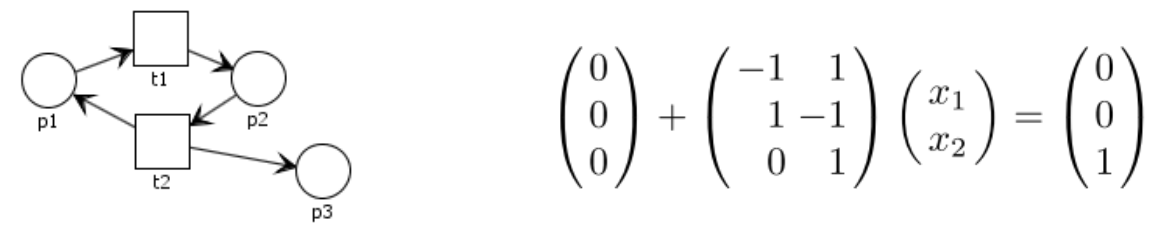
\includegraphics[width=0.6\textwidth]{algebraicAnalysisFail.png}
\end{center}

Тут вектор $(1, 1)$, очевидно, является решением уравнения состояния, но эта сеть, изначально не имеющая маркеров, очевидно, маркер произвести никак не может. Почему так --- потому что уравнение состояния никак не учитывает последовательности срабатываний, а следовательно, и живости переходов в момент, когда по мнению уравнения состояния переход должен сработать. Если бы в примере выше переходы реально могли сработать, сеть бы оказалась в нужном состоянии без проблем, но они не могут.

Поэтому алгебраический способ подходит только, чтобы быстро проверить, может ли выполняться доказываемое свойство вообще. Если да, то может применяться структурный анализ --- это когда мы выделяем в сети некоторые структурные элементы (например, \textit{сифоны}, то есть куски сети, которые производят токены, и \textit{ловушки}, которые токены поглощают), и смотрим, как они соотносятся друг с другом. Либо анализ редукцией --- когда мы упрощаем сеть, склеивая состояния и переходы, которые можно склеить, по следующим правилам:

\begin{center}
    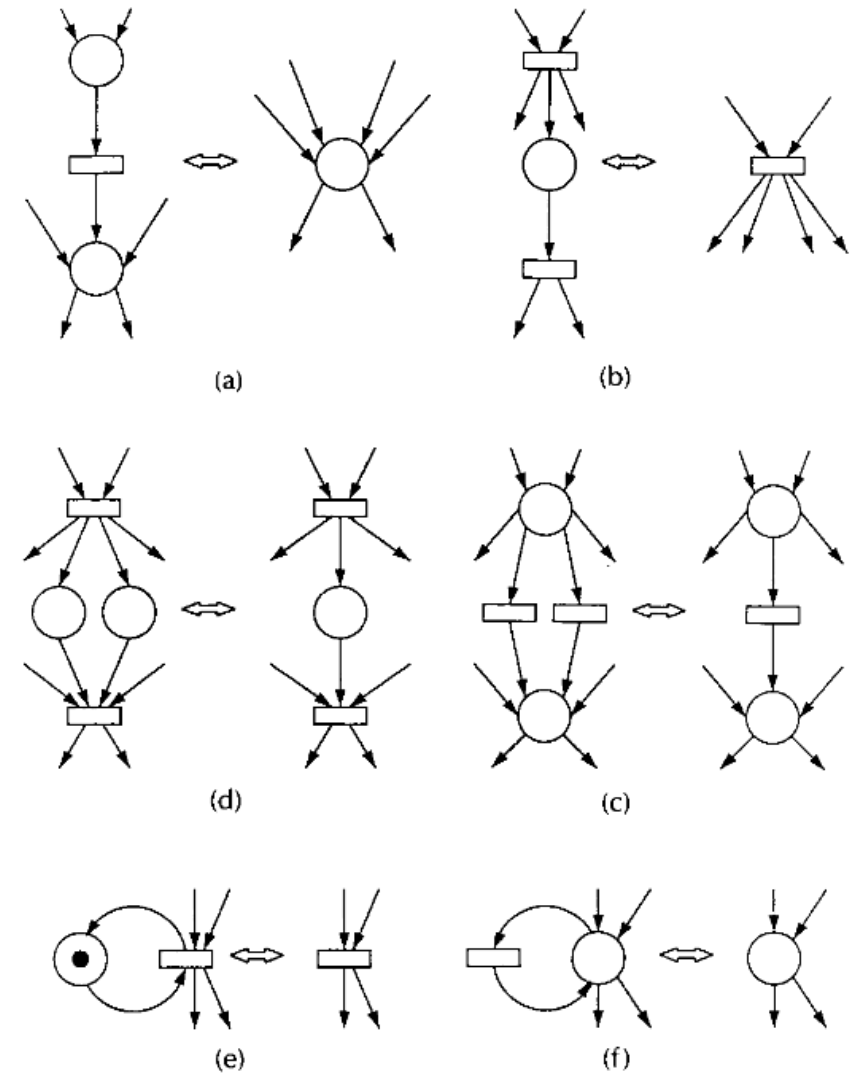
\includegraphics[width=0.5\textwidth]{petriReduction.png}
    \attribution{Murata Tadao. Petri nets: Properties, analysis and applications}
\end{center}

Этот способ сам по себе редко что-то даёт, но его имеет смысл применять, чтобы упростить сеть и тем самым уменьшить размер задачи для самого мощного и самого трудоёмкого способа анализа сети: метода анализа пространства состояний.

Метод заключается в построении дерева (или графа) всех возможных состояний, которые могут быть получены переходами из данного:

\begin{center}
    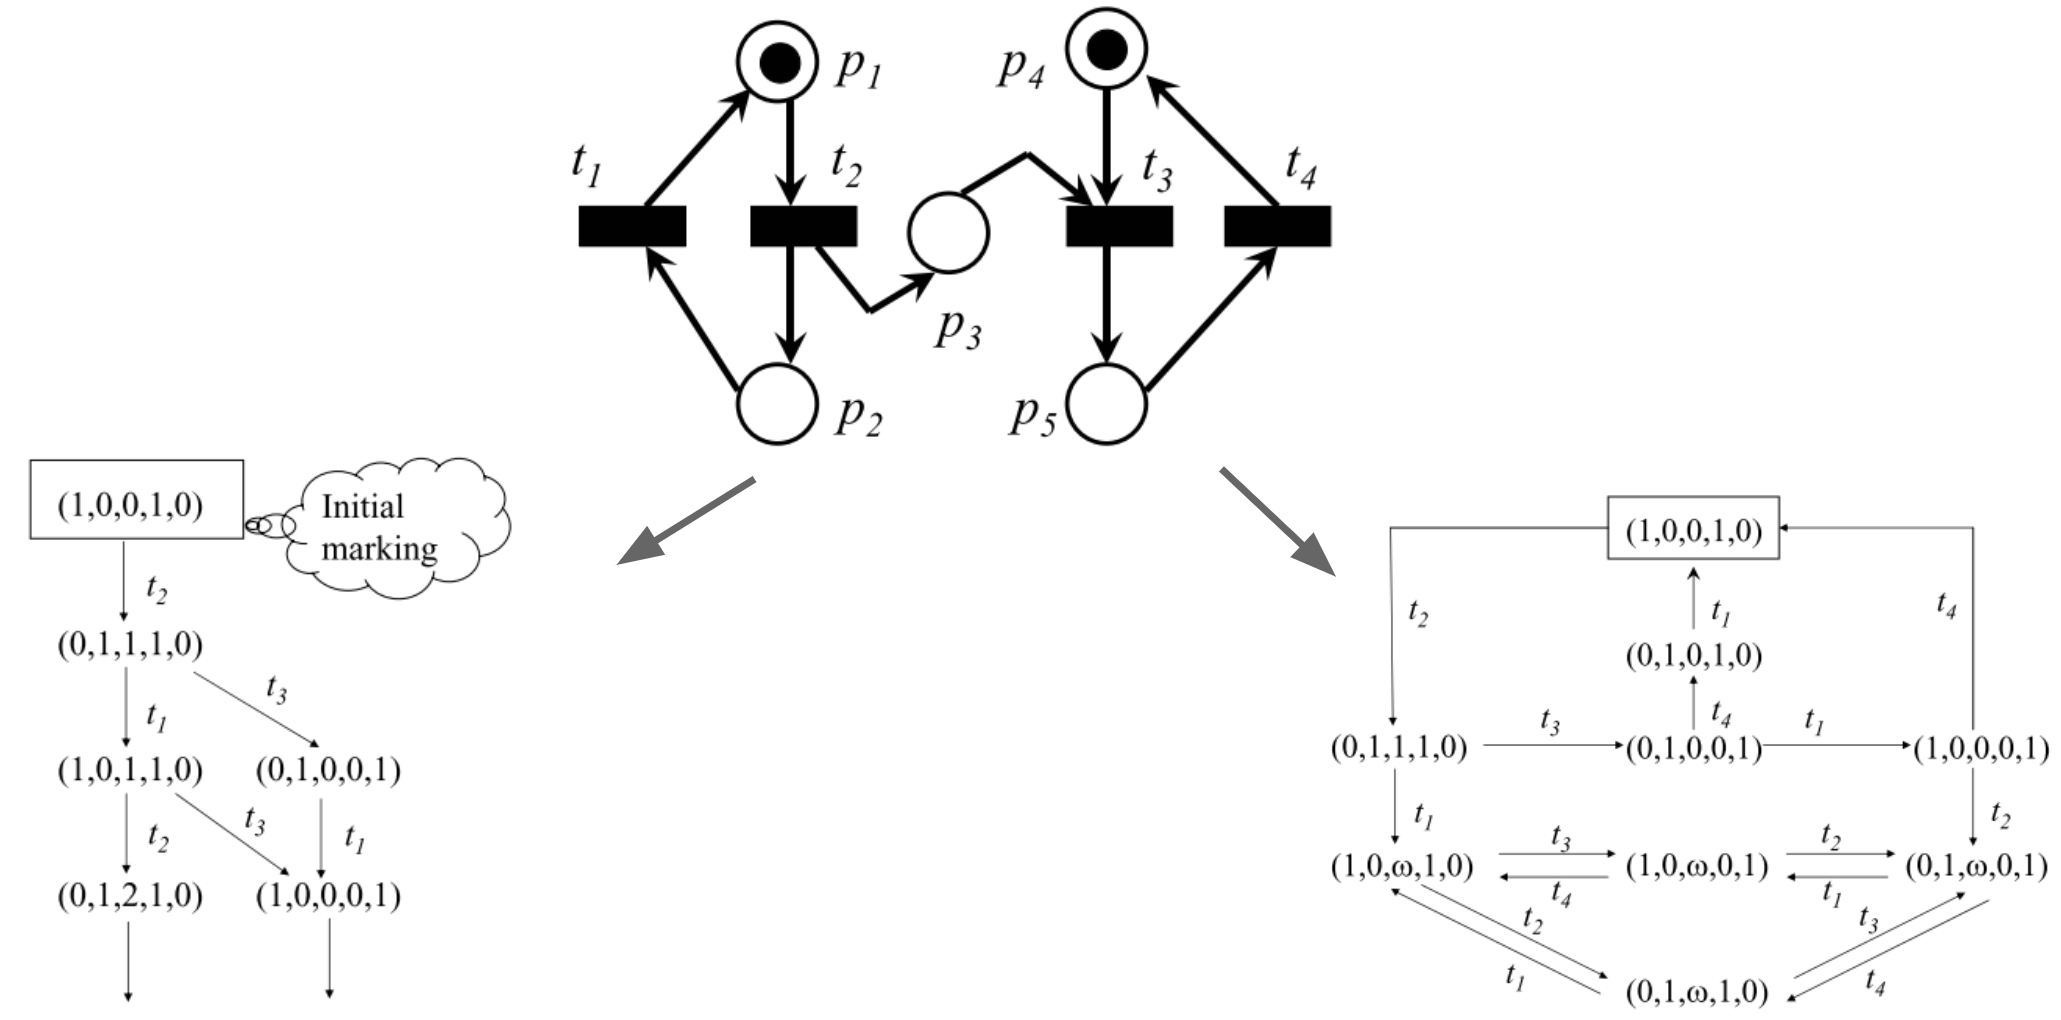
\includegraphics[width=\textwidth]{petriStateSpaceAnalysis.png}
\end{center}

Из каждого состояния (то бишь маркировки сети) ведут рёбра, соответствующие живым переходам в новое состояние (то бишь маркировку, полученную переходом). Дерево обладает тем неприятным (но ожидаемым) свойством, что оно бесконечно для подавляющего большинства сетей, поэтому чаще рассматривают граф переходов. В графе неограниченные состояния (то есть состояния, в которых в одном из мест может быть сколько угодно токенов) записываются с использованием символа $\omega$. Например, из состояния $(0, 1, 1, 1, 0)$ можно попасть в $(1, 0, 1, 1, 0)$, из него в $(0, 1, 2, 1, 0)$. И тут мы замечаем, что $(0, 1, 2, 1, 0)$ \textit{покрывает} состояние $(0, 1, 1, 1, 0)$, то есть в нём количество токенов во всех местах сети больше либо равно, чем в состоянии $(0, 1, 1, 1, 0)$. Это означает, что во всех местах, в которых токенов строго больше, может быть бесконечно много токенов (в нашем примере это соответствует ситуации, когда производитель производит данные быстрее, чем потребитель успевает их обрабатывать), так что все такие состояния можно склеить в одно, считая количество токенов в <<плохих>> местах равным $\omega$ (которое означает <<сколь угодно много>>). Граф состояний всегда конечен.

Анализ пространства состоянии позволяет точно доказать или опровергнуть очень многие свойства сети, но имеет один важный недостаток --- экспоненциальный рост числа маркировок при росте числа мест и переходов сети (даже в случае использования графа, который не так-то тривиально построить). Но по сравнению с машинами Тьюринга, для которых любое нетривиальное свойство скорее всего вообще алгоритмически неразрешимо, это считается успехом, и в сообществе, занимающемся сетями Петри, искренне радуются новым алгоритмам с экспоненциальной трудоёмкостью.

\subsection{Примеры использования}

Закончим мы парой примеров использования сетей Петри в программировании, взятых из научных статей (вообще, в научном сообществе сети Петри всё ещё очень популярны, несмотря на то, что, казалось бы, всё, что про них можно было сказать, было сказано ещё в начале 90-х). 

Первый пример из статьи G. Chang, D. Kulić <<Robot Task Learning from Demonstration Using Petri Nets>> 2013-го года. Там сети Петри использовались как способ хранения и представления знаний. Роботу с камерой показывают, как выполнять то или иное действие (например, переложить цветные параллелепипеды в правильном порядке), он строит сеть Петри, соединяющую состояния наблюдаемых объектов и действия (переходы). Потом воспроизводит последовательность действий от начального состояния к заданному. При этом, в чём тут преимущество сетей Петри, робот может сам найти решение похожей задачи (или подзадачи) путём поиска по дереву состояний:

\begin{center}
    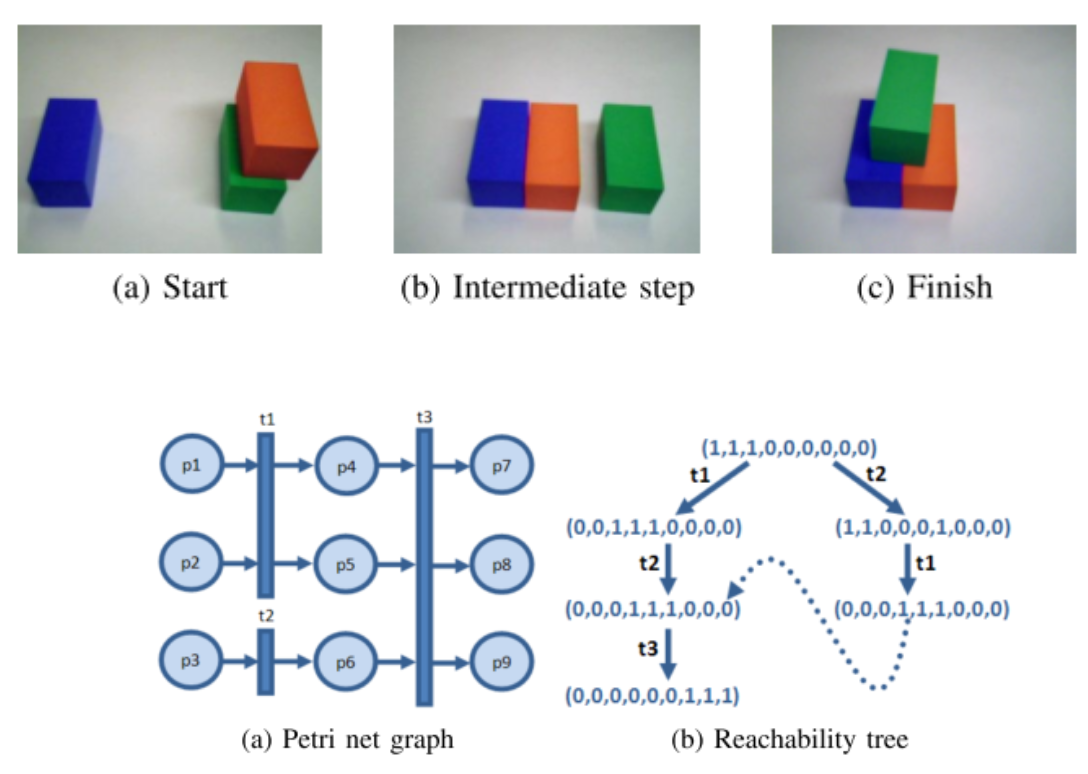
\includegraphics[width=0.8\textwidth]{petriUsageExample1.png}
    \attribution{G. Chang, D. Kulić. Robot Task Learning from Demonstration Using Petri Nets}
\end{center}

Состояний обычно не очень много, так что перебор пространства состояний не занимает много времени. И позволяет решить проблему, сформулированную в анекдоте <<Как программисту вскипятить чайник? Налить воды, поставить на огонь, подождать пока вскипит. А если в чайнике уже есть вода? Вылить воду и свести задачу к предыдущей.>>.

Второй пример --- из статьи 2007 года Y.T. Kotb et al. <<Petri Net-Based Cooperation In Multi-Agent Systems>>. Это тоже была статья про роботов, но на сей раз роботов много и все они обладают разными возможностями --- например, у кого-то есть манипулятор, кто-то может перевозить грузы. Задача --- обеспечить совместное достижение группой роботов некоторой цели, с автоматическим распределением задач между роботами. Решение --- представим деятельность каждого робота в виде сети Петри, где переходам будут соответствовать действия, а местам --- состояния робота. Заведём промежуточные места и переходы, отвечающие точкам синхронизации роботов, и будем искать на пространстве состояний пути, которые быстрее всего приведут к целевому состоянию:

\begin{center}
    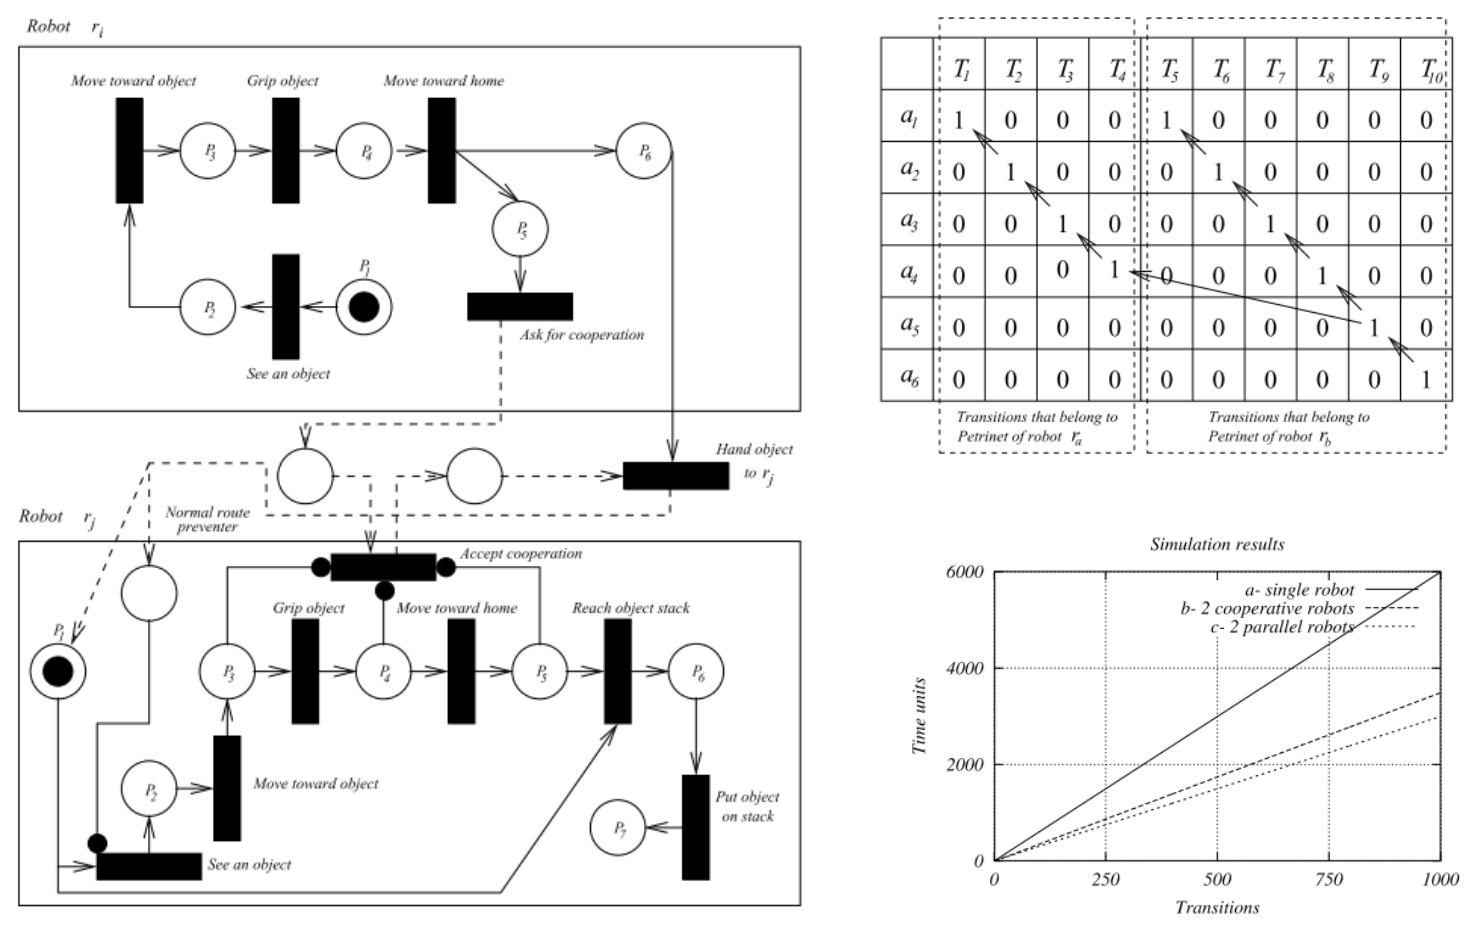
\includegraphics[width=0.9\textwidth]{petriUsageExample2.png}
    \attribution{Y.T. Kotb et al. Petri Net-Based Cooperation In Multi-Agent Systems}
\end{center}

\section{Литература}

\noindent\begin{minipage}{\textwidth}
    \begin{minipage}[c][6cm][c]{\dimexpr0.7\textwidth-0.5\Colsep\relax}
        На этом заканчивается обзор языков визуального моделирования. Для закрепления знаний очень рекомендую книжку М. Фаулер, UML. Основы. Краткое руководство по стандартному языку объектного моделирования. СПб., Символ-Плюс, 2011. 192 С. Книжка короткая, состоит в основном из картинок, но содержит, в целом, все знания, которые нужны, чтобы использовать на практике UML-диаграммы.
    \end{minipage}\hfill
    \begin{minipage}[c][6cm][c]{\dimexpr0.3\textwidth-0.5\Colsep\relax}
        
\includegraphics[width=0.6\textwidth]{umlBookCover.png}
    \end{minipage}%
\end{minipage}

\end{document}
